% !TEX program = xelatex
% Build: latexmk -xelatex -interaction=nonstopmode -halt-on-error cs229s_project1_report.tex
% Figures: python solutions/cs229s/project1-transformer-kernels/scripts/plot_gpu.py (read from the lab's artifacts/figures)
% Every number below is copied from solutions/cs229s/project1-transformer-kernels/artifacts/raw/{*.csv,gpu/*.jsonl}
\documentclass[11pt,a4paper]{ctexart}
% Shared preamble for the assignment reports. Use with:
%   \documentclass[11pt,a4paper]{ctexart}  (XeLaTeX)
%   % Shared preamble for the assignment reports. Use with:
%   \documentclass[11pt,a4paper]{ctexart}  (XeLaTeX)
%   % Shared preamble for the assignment reports. Use with:
%   \documentclass[11pt,a4paper]{ctexart}  (XeLaTeX)
%   \input{../common/preamble.tex}
\usepackage[margin=2.3cm]{geometry}
\setmainfont{texgyretermes}[Extension=.otf,UprightFont=*-regular,BoldFont=*-bold,ItalicFont=*-italic,BoldItalicFont=*-bolditalic]
\setsansfont{texgyreheros}[Extension=.otf,UprightFont=*-regular,BoldFont=*-bold,ItalicFont=*-italic,BoldItalicFont=*-bolditalic]
\setmonofont{texgyrecursor}[Extension=.otf,UprightFont=*-regular,BoldFont=*-bold,ItalicFont=*-italic,BoldItalicFont=*-bolditalic]
\usepackage{amsmath,amssymb,mathtools,bm}
\usepackage{graphicx}
\usepackage{booktabs,multirow,makecell,array,tabularx}
\usepackage[table]{xcolor}
\usepackage[most]{tcolorbox}
\usepackage{enumitem}
\usepackage{listings}
\usepackage{subcaption}
\usepackage{siunitx}
\usepackage[hidelinks]{hyperref}
\usepackage[nameinlink,noabbrev]{cleveref}
\usepackage{float}

\setlength{\emergencystretch}{3em}
\linespread{1.15}
\setlist{leftmargin=*,itemsep=2pt,topsep=3pt}
\graphicspath{{figures/}}

\crefname{figure}{图}{图}
\crefname{table}{表}{表}
\crefname{section}{第}{第}
\creflabelformat{section}{#2#1#3 节}
\crefname{equation}{式}{式}
\crefformat{equation}{式~(#2#1#3)}

\lstset{basicstyle=\ttfamily\footnotesize,columns=fullflexible,breaklines=true,frame=single,
  framerule=0.3pt,rulecolor=\color{black!40},backgroundcolor=\color{black!3},
  keywordstyle=\color{blue!60!black}\bfseries,commentstyle=\color{green!40!black},
  numbers=left,numberstyle=\tiny\color{black!50},xleftmargin=1.5em}

% Interview boxes: question, model answer, common wrong answer.
\newtcolorbox{iqbox}[1]{enhanced,breakable,colback=blue!3,colframe=blue!45!black,boxrule=0.5pt,arc=1.5pt,
  left=4pt,right=4pt,top=3pt,bottom=3pt,fonttitle=\bfseries\small,title={面试追问：#1}}
\newtcolorbox{findingbox}[1][]{enhanced,breakable,colback=green!3,colframe=green!40!black,boxrule=0.5pt,arc=1.5pt,
  left=4pt,right=4pt,top=3pt,bottom=3pt,fonttitle=\bfseries\small,title={结论#1}}
\newtcolorbox{caveatbox}{enhanced,breakable,colback=orange!4,colframe=orange!60!black,boxrule=0.5pt,arc=1.5pt,
  left=4pt,right=4pt,top=3pt,bottom=3pt,fonttitle=\bfseries\small,title={不能推出的结论}}

\newcommand{\authorline}{ShaneLiu04\thanks{GitHub: \url{https://github.com/ShaneLiu04}。代码与原始指标：\url{https://gitee.com/liu-xingyan04/mlsys-infra}。本文基于公开课程材料独立完成，与课程团队无隶属关系。}}

\usepackage[margin=2.3cm]{geometry}
\setmainfont{texgyretermes}[Extension=.otf,UprightFont=*-regular,BoldFont=*-bold,ItalicFont=*-italic,BoldItalicFont=*-bolditalic]
\setsansfont{texgyreheros}[Extension=.otf,UprightFont=*-regular,BoldFont=*-bold,ItalicFont=*-italic,BoldItalicFont=*-bolditalic]
\setmonofont{texgyrecursor}[Extension=.otf,UprightFont=*-regular,BoldFont=*-bold,ItalicFont=*-italic,BoldItalicFont=*-bolditalic]
\usepackage{amsmath,amssymb,mathtools,bm}
\usepackage{graphicx}
\usepackage{booktabs,multirow,makecell,array,tabularx}
\usepackage[table]{xcolor}
\usepackage[most]{tcolorbox}
\usepackage{enumitem}
\usepackage{listings}
\usepackage{subcaption}
\usepackage{siunitx}
\usepackage[hidelinks]{hyperref}
\usepackage[nameinlink,noabbrev]{cleveref}
\usepackage{float}

\setlength{\emergencystretch}{3em}
\linespread{1.15}
\setlist{leftmargin=*,itemsep=2pt,topsep=3pt}
\graphicspath{{figures/}}

\crefname{figure}{图}{图}
\crefname{table}{表}{表}
\crefname{section}{第}{第}
\creflabelformat{section}{#2#1#3 节}
\crefname{equation}{式}{式}
\crefformat{equation}{式~(#2#1#3)}

\lstset{basicstyle=\ttfamily\footnotesize,columns=fullflexible,breaklines=true,frame=single,
  framerule=0.3pt,rulecolor=\color{black!40},backgroundcolor=\color{black!3},
  keywordstyle=\color{blue!60!black}\bfseries,commentstyle=\color{green!40!black},
  numbers=left,numberstyle=\tiny\color{black!50},xleftmargin=1.5em}

% Interview boxes: question, model answer, common wrong answer.
\newtcolorbox{iqbox}[1]{enhanced,breakable,colback=blue!3,colframe=blue!45!black,boxrule=0.5pt,arc=1.5pt,
  left=4pt,right=4pt,top=3pt,bottom=3pt,fonttitle=\bfseries\small,title={面试追问：#1}}
\newtcolorbox{findingbox}[1][]{enhanced,breakable,colback=green!3,colframe=green!40!black,boxrule=0.5pt,arc=1.5pt,
  left=4pt,right=4pt,top=3pt,bottom=3pt,fonttitle=\bfseries\small,title={结论#1}}
\newtcolorbox{caveatbox}{enhanced,breakable,colback=orange!4,colframe=orange!60!black,boxrule=0.5pt,arc=1.5pt,
  left=4pt,right=4pt,top=3pt,bottom=3pt,fonttitle=\bfseries\small,title={不能推出的结论}}

\newcommand{\authorline}{ShaneLiu04\thanks{GitHub: \url{https://github.com/ShaneLiu04}。代码与原始指标：\url{https://gitee.com/liu-xingyan04/mlsys-infra}。本文基于公开课程材料独立完成，与课程团队无隶属关系。}}

\usepackage[margin=2.3cm]{geometry}
\setmainfont{texgyretermes}[Extension=.otf,UprightFont=*-regular,BoldFont=*-bold,ItalicFont=*-italic,BoldItalicFont=*-bolditalic]
\setsansfont{texgyreheros}[Extension=.otf,UprightFont=*-regular,BoldFont=*-bold,ItalicFont=*-italic,BoldItalicFont=*-bolditalic]
\setmonofont{texgyrecursor}[Extension=.otf,UprightFont=*-regular,BoldFont=*-bold,ItalicFont=*-italic,BoldItalicFont=*-bolditalic]
\usepackage{amsmath,amssymb,mathtools,bm}
\usepackage{graphicx}
\usepackage{booktabs,multirow,makecell,array,tabularx}
\usepackage[table]{xcolor}
\usepackage[most]{tcolorbox}
\usepackage{enumitem}
\usepackage{listings}
\usepackage{subcaption}
\usepackage{siunitx}
\usepackage[hidelinks]{hyperref}
\usepackage[nameinlink,noabbrev]{cleveref}
\usepackage{float}

\setlength{\emergencystretch}{3em}
\linespread{1.15}
\setlist{leftmargin=*,itemsep=2pt,topsep=3pt}
\graphicspath{{figures/}}

\crefname{figure}{图}{图}
\crefname{table}{表}{表}
\crefname{section}{第}{第}
\creflabelformat{section}{#2#1#3 节}
\crefname{equation}{式}{式}
\crefformat{equation}{式~(#2#1#3)}

\lstset{basicstyle=\ttfamily\footnotesize,columns=fullflexible,breaklines=true,frame=single,
  framerule=0.3pt,rulecolor=\color{black!40},backgroundcolor=\color{black!3},
  keywordstyle=\color{blue!60!black}\bfseries,commentstyle=\color{green!40!black},
  numbers=left,numberstyle=\tiny\color{black!50},xleftmargin=1.5em}

% Interview boxes: question, model answer, common wrong answer.
\newtcolorbox{iqbox}[1]{enhanced,breakable,colback=blue!3,colframe=blue!45!black,boxrule=0.5pt,arc=1.5pt,
  left=4pt,right=4pt,top=3pt,bottom=3pt,fonttitle=\bfseries\small,title={面试追问：#1}}
\newtcolorbox{findingbox}[1][]{enhanced,breakable,colback=green!3,colframe=green!40!black,boxrule=0.5pt,arc=1.5pt,
  left=4pt,right=4pt,top=3pt,bottom=3pt,fonttitle=\bfseries\small,title={结论#1}}
\newtcolorbox{caveatbox}{enhanced,breakable,colback=orange!4,colframe=orange!60!black,boxrule=0.5pt,arc=1.5pt,
  left=4pt,right=4pt,top=3pt,bottom=3pt,fonttitle=\bfseries\small,title={不能推出的结论}}

\newcommand{\authorline}{ShaneLiu04\thanks{GitHub: \url{https://github.com/ShaneLiu04}。代码与原始指标：\url{https://gitee.com/liu-xingyan04/mlsys-infra}。本文基于公开课程材料独立完成，与课程团队无隶属关系。}}

\graphicspath{{../../solutions/cs229s/project1-transformer-kernels/artifacts/figures/}}

\title{CS229S Project 1 实验报告：\\Transformer 内核、IO 模型与 RTX 5090 上的实测}
\author{\authorline}
\date{2026 年 10 月}

\begin{document}
\maketitle

\begin{abstract}
本文对应 Stanford CS229S（Fall 2023）Project 1。原有实验是 CPU/numpy 版：分块 FlashAttention 前向与反向、HBM 流量（IO）模型、
depthwise 因果卷积的几种写法、以及手工设定权重的两层 associative recall transformer。本次在 RTX 5090（sm\_120，170 SM，32 GB GDDR7，96 MB L2）上补齐 GPU 部分：
(1) 用 Triton 写 FlashAttention-2 的前向和反向，与朴素 PyTorch（显式物化 $S,P$）以及 \texttt{scaled\_dot\_product\_attention} 的 flash / efficient / math 三个后端对比，
扫描 $T=256\ldots32768$、$d\in\{64,128\}$、因果/非因果、fp16/bf16；(2) 实测 copy 带宽（1.52 TB/s）与 BF16 矩阵乘峰值（236.3 TFLOP/s），
把 Llama-2-7B 一层的 QKV 投影、attention、输出投影、MLP 在 prefill 与 decode 形状下画到 roofline 上；(3) 写三个 depthwise 1D 卷积 CUDA kernel（一线程一输出、共享内存 + halo、寄存器分块），
与 cuDNN \texttt{conv1d(groups=C)} 和 FFT 卷积对比，核长从 3 扫到 8192；(4) 在 GPU 上训练小 GPT 解 MQAR，测 tokens/s 与 MFU。

主要结论：Triton 前向在长序列上与 PyTorch 自带的 FlashAttention-2 持平（fp16、$d=64$、$T=16384$：224.0 对 217.9 TFLOP/s），
比朴素实现快 7.15 倍（$T=8192$ 非因果）到 22.2 倍（因果）；朴素实现与 math 后端在 $B\cdot H=32$、$T=16384$ 时 OOM，而 flash 类方法在 $T=32768$ 时额外显存只有 138 MB。
朴素实现的耗时可以用「eager 实现的 $6T^2$ 次 fp16 读写 ÷ copy 带宽」解释到 93\%；而按 IO 模型计算 FlashAttention 的「隐含带宽」最高达 6.57 TB/s，
是 DRAM 带宽的 4.3 倍——K/V 的重复读取大部分命中了 96 MB L2，教科书的 $\Theta(T^2d^2/M)$ 只给出了 DRAM 流量的上界。
寄存器分块的卷积 kernel 在 $K=1024$ 时达到 45.0 TFLOP/s（直接卷积等效），比 cuDNN 快 6.5 倍，并在 $N=16384$ 时仍快于 FFT；短卷积 $K=4$ 时它达到 copy 带宽的 97\%。
训练方面，2 层 GPT 在 MQAR 上于第 1000–1100 步从 0.17 的平台突然跳到 100\%，1 层模型学不会；用本文 Triton kernel（含反向）训练的学习曲线与 SDPA 重合。
GPT-2-small 形状下 bf16 + SDPA 达到 159.6k tokens/s、MFU 0.447，是 fp32 朴素实现的 3.84 倍。
\end{abstract}

\tableofcontents
\clearpage

%======================================================================
\section{背景与作业要求}
%======================================================================

CS229S Project 1 由四个官方部分组成，本文逐一对应如下（\cref{tab:map}）。FlashAttention 不是官方必做项，但第 3 部分「分析多头注意力的算术强度」
需要一个能测的 attention kernel，所以把它作为 GPU 部分的主线。

\begin{table}[H]
\centering\small
\caption{官方作业与本文实现的对应关系}\label{tab:map}
\begin{tabularx}{\linewidth}{>{\raggedright\arraybackslash}p{3.2cm}>{\raggedright\arraybackslash}X>{\raggedright\arraybackslash}p{3.6cm}}
\toprule
官方部分 & 本文实现 & 位置 \\
\midrule
1. 训练一个小 Transformer & GPU 上训练 1/2 层 GPT 解 MQAR（多查询 associative recall），比较 bf16 autocast、SDPA flash、朴素 attention、自写 Triton attention；GPT-2-small 形状测 tokens/s 与 MFU & \cref{sec:train} \\
2. 手写两层 Transformer 解 associative recall & CPU 部分：上一 token 头 + 匹配头，权重全部手工设定；本次在 GPU 上复核，24 组配置与 CPU 预测完全一致 & \cref{sec:cpu,sec:recallgpu} \\
3. MHA 的算术强度 & CPU 部分：朴素/flash 的 HBM 字节模型、decode 阶段 MHA/GQA/MQA 强度；GPU 部分：实测 roofline，Llama-2-7B 一层四个算子在 prefill/decode 形状下的位置 & \cref{sec:roof,sec:theory} \\
4. 1D depthwise 卷积 CUDA kernel & CPU 部分：numpy 的四种写法；GPU 部分：三个 CUDA kernel（naive / smem+halo / 寄存器分块）对比 cuDNN 与 FFT & \cref{sec:conv} \\
（补充）FlashAttention & CPU：numpy 分块前向/反向 + IO 计数器；GPU：Triton 前向 + 反向，块大小扫描 & \cref{sec:flash} \\
\bottomrule
\end{tabularx}
\end{table}

%======================================================================
\section{实验环境}
%======================================================================

\begin{table}[H]
\centering\small
\caption{软硬件环境（GPU 信息来自 \texttt{attention\_fwd.jsonl} 的 meta 行，CPU 信息来自 \texttt{meta.json}）}
\begin{tabularx}{\linewidth}{lX}
\toprule
GPU & NVIDIA GeForce RTX 5090，compute capability 12.0（sm\_120），170 SM，33.67 GB 可见显存，96 MB L2；
规格：GDDR7 1.792 TB/s，dense BF16 张量核 209.5 TFLOP/s（boost 时钟下）\\
GPU 软件 & Python 3.12.3，PyTorch 2.8.0+cu128，Triton 3.4.0，CUDA 12.8（nvcc \texttt{-arch=sm\_120}），cuDNN 9.10.2 \\
GPU 主机 & AutoDL 容器，7 个任务共享；本文所有 GPU 计时都在共享锁 \texttt{flock gpu.lock} 内独占 GPU 完成，CPU 绑定在 2 个核（\texttt{taskset -c 38,40}）\\
CPU 部分 & Windows Server，Intel Ice Lake（Family 6 Model 106），4 物理核 / 8 逻辑核，与其他任务共享；Python 3.12.10，numpy 2.5.3，torch 2.6.0 CPU \\
实测峰值 & copy 带宽 1521.9 GB/s（2 GiB 缓冲），只读求和 1625.6 GB/s；BF16 \texttt{matmul} 峰值 236.3 TFLOP/s（$n=6144$），fp16 220.3，TF32 113.8，fp32 65.7；ridge point $236.3/1.522=155.3$ FLOP/B \\
\bottomrule
\end{tabularx}
\end{table}

实测 BF16 峰值比规格高 13\%。原因是规格按 2.41 GHz boost 时钟计算，而这块卡的最高 SM 时钟是 3090 MHz（\texttt{nvidia-smi} 的 \texttt{clocks.max.sm}），
持续负载下时钟高于标称 boost。本文 roofline 与 MFU 的分母一律用实测值（236.3 TFLOP/s、1.522 TB/s），图中同时画出规格屋顶作参照。
ncu 在该容器中报 \texttt{ERR\_NVGPUCTRPERM}（无权读取性能计数器，记录在 \texttt{ncu\_attention.jsonl}），所以本文没有 DRAM 字节的直接测量，
只能用「模型字节 ÷ 实测时间」得到的隐含带宽去推断（\cref{sec:blocks}）。

%======================================================================
\section{方法与实现}
%======================================================================

\subsection{Triton FlashAttention-2 前向}\label{sec:impl-fwd}

算法来自 FlashAttention\cite{fa1} 与 FlashAttention-2\cite{fa2}（外层循环为 Q 块），online softmax 来自 \cite{online,rabe}，用 Triton\cite{triton} 实现。
每个 Triton program 负责一个 $(Q\text{ 块}, b\cdot h)$：把 $B_r$ 行 $Q$ 读进寄存器/共享内存，沿 K/V 方向以 $B_c$ 为步长循环，维护行最大值 $m$、归一化因子 $\ell$ 与未归一化输出 $\mathrm{acc}$。
三个实现细节：
\begin{enumerate}
\item \textbf{以 2 为底的 online softmax}：把 $\log_2 e$ 并入缩放系数，用 \texttt{exp2} 代替 \texttt{exp}（GPU 上 \texttt{ex2.approx} 是单条 SFU 指令）。最后存 $\mathrm{lse}=(m+\log_2\ell)\ln 2$ 供反向使用。
\item \textbf{因果掩码分两段}：对角线左侧的整块不需要掩码；只有跨对角线的块做 \texttt{tl.where}；对角线右上方的块根本不加载。
  对角段的起点取 $\lfloor sB_r/B_c\rfloor B_c$，这样任意 $B_r,B_c$ 组合都正确（测试覆盖 $B_r<B_c$ 的情况）。
\item \textbf{反向调度}：因果时 program 0 处理最后一个 Q 块（工作量最大），减少尾部不均衡。
\end{enumerate}

\begin{lstlisting}[language=Python,caption={前向内层循环（\texttt{gpu/flash\_triton.py}，有删节）}]
for start_n in range(lo, hi, BLOCK_N):
    cols = start_n + offs_n
    k = tl.load(k_base + cols[None, :] * HEAD_DIM + offs_d[:, None])     # (D, Bc)
    qk = tl.dot(q, k) * qk_scale                       # qk_scale = sm_scale * log2(e)
    if MASK_CAUSAL:
        qk = tl.where(offs_m[:, None] >= cols[None, :], qk, float("-inf"))
    m_new = tl.maximum(m_i, tl.max(qk, 1))
    alpha = tl.math.exp2(m_i - m_new)                  # rescale old state
    p = tl.math.exp2(qk - m_new[:, None])
    l_i = l_i * alpha + tl.sum(p, 1)
    v = tl.load(v_base + cols[:, None] * HEAD_DIM + offs_d[None, :])     # (Bc, D)
    acc = tl.dot(p.to(v.dtype), v, acc * alpha[:, None])
    m_i = m_new
\end{lstlisting}

默认配置（按顺序尝试，直到共享内存放得下）：$d=64$ 用 $(B_r,B_c,\text{warps},\text{stages})=(128,64,4,3)$，$d=128$ 用 $(128,64,8,2)$。
sm\_120 每个 block 最多 99 KB 共享内存（比 H100 的 227 KB 小得多），$d=128$ 时 $Q$ 块 32 KB 加两级流水的 K/V 共 64 KB 刚好放下，三级就放不下了。

\subsection{Triton 反向}\label{sec:impl-bwd}

反向与 CPU 版 \texttt{flash\_backward} 同构：先用 PyTorch 算 $D_i=\sum_j dO_{ij}O_{ij}$，然后两个 kernel。
\texttt{\_attn\_bwd\_dkdv} 每个 program 持有一个 K/V 块，沿 Q 方向循环，重算 $P^\top=\exp(KQ^\top\cdot s-\mathrm{lse})$，累加 $dV\mathrel{+}=P^\top dO$、$dK\mathrel{+}=dS^\top Q$；
\texttt{\_attn\_bwd\_dq} 每个 program 持有一个 Q 块，沿 K/V 方向循环累加 $dQ\mathrel{+}=dS\,K$。两者都不写 $P$，也没有原子操作。
代价是 $QK^\top$ 和 $dO\,V^\top$ 各被重算两次（FA2 原文用一个 kernel 加原子累加 $dQ$，或像 Triton 官方教程那样在一个 kernel 里同时做两件事），所以反向比 PyTorch 的 FA2 慢约 20\%（\cref{sec:bwd}）。

\subsection{计时与正确性方法}
\begin{itemize}
\item 计时：CUDA event，先预热 2–5 次，取 10–30 次的中位数；单次测量时长上限 1.5 s。
\item 峰值显存：调用前 \texttt{reset\_peak\_memory\_stats}，报告 \texttt{max\_memory\_allocated} 减去调用前已分配量（即「输入之外的额外显存」）。OOM 被捕获并记录，之后更长的 $T$ 直接标记为 \texttt{skipped\_after\_oom}。
\item 误差：对 batch 0、head 0 用 fp32 分块参考实现（按 query 分块，显存 $O(2048\cdot T)$）计算 $\max|O-O_{\text{fp32}}|$；反向梯度对前 2 个 head 用 fp32 的 math 后端 autograd 作参考（$T\le4096$）。
\item FLOPs：前向 $4BHT^2d$，因果只计有用的一半；前向+反向按 FA2 论文记为前向的 3.5 倍（反向 5 个矩阵乘对前向 2 个）。
\end{itemize}

\subsection{Roofline 与一层 Llama-2-7B}
copy 带宽用 \texttt{y.copy\_(x)}（读 + 写）扫 64 KiB–2 GiB；峰值取 $\ge256$ MiB（远超 96 MB L2）的最大值。BF16 峰值取方阵乘 $n=256\ldots16384$ 的最大值。
Roofline 模型见 \cite{roofline}。一层的四个算子用 Llama-2-7B\cite{llama2} 的形状（$d=4096$，32 头，$d_h=128$，$d_{ff}=11008$，gated MLP），bf16：
QKV 投影 $[M,d]\times[d,3d]$；attention 用 SDPA 的 flash/efficient 后端；输出投影 $[M,d]\times[d,d]$；MLP 为 $[M,d]\times[d,2d_{ff}]$、\texttt{silu}$\cdot$、$[M,d_{ff}]\times[d_{ff},d]$。
FLOPs 与字节一律用 \texttt{tools/mlsys\_calc.py} 的 \texttt{gemm\_intensity}（每个矩阵过一次 HBM）和 \texttt{kv\_cache\_bytes}，
所以图上的横坐标就是解析强度，纵坐标是实测吞吐。prefill 取 $B=1$、$T\in\{128,512,2048,8192\}$ 与 $B=8,T=2048$；decode 取上下文 4096、$B\in\{1,4,16,64,256\}$。

\subsection{Depthwise 卷积的三个 CUDA kernel}\label{sec:impl-conv}

$y[b,c,t]=\sum_{j<K}h[c,j]\,x[b,c,t-j]$，fp32，通过 \texttt{torch.utils.cpp\_extension.load\_inline} 编译（\texttt{-O3 -arch=sm\_120}）。
\begin{itemize}
\item \textbf{naive}：一线程一输出，$K$ 次全局读 $x$ 和 $h$，复用全靠 L1/L2。
\item \textbf{smem}：（H3/Hyena\cite{h3,hyena} 与 Mamba\cite{mamba} 中的短/长卷积都是这个算子）一个 block 负责一行 $(b,c)$ 的 256 个输出，把 $x[t_0-K+1,\,t_0+256)$（含 $K-1$ 的 halo）和 $h[c,:]$ 搬进共享内存。每个 FMA 仍要 2 次共享内存读（$h_j$ 是广播，$x$ 是连续地址，无 bank 冲突）。
\item \textbf{regblock}：每线程负责 $R=8$ 个连续输出，抽头按 $R$ 个一组处理：先把 $2R-1$ 个 $x$ 读进寄存器窗口 $w$，再做 $R\times R$ 个 FMA，所以 64 个 FMA 只要 23 次共享内存读。
  线程 $i$ 读 \texttt{sx[8i+c]} 本会 8 路 bank 冲突，用 \texttt{PADI(i)=i+(i>>5)} 的填充下标消除；输出先写回共享内存再合并写出全局内存。
\end{itemize}

\begin{lstlisting}[language=C++,caption={寄存器分块 kernel 的核心循环（\texttt{gpu/dwconv\_cuda.py}）}]
for (int jb = 0; jb < Kp; jb += R) {               // taps in chunks of R (h zero-padded to Kp)
  const int base = o0 + Kp - jb - R;
  float w[2 * R - 1];
#pragma unroll
  for (int i = 0; i < 2 * R - 1; ++i) w[i] = sx[PADI(base + i)];
#pragma unroll
  for (int jj = 0; jj < R; ++jj) {
    const float hv = sh[jb + jj];                  // broadcast
#pragma unroll
    for (int r = 0; r < R; ++r) acc[r] = fmaf(hv, w[r - jj + R - 1], acc[r]);
  }
}
\end{lstlisting}

\subsection{训练}
\texttt{gpu/tiny\_gpt.py} 是一个 pre-LN GPT（可学习位置编码，输入输出嵌入共享），attention 实现可切换为 \texttt{naive}、\texttt{sdpa}（自动选 flash）或 \texttt{triton}（本文的 kernel，前向 + 反向）。
MQAR 任务（Zoology\cite{zoology}）：序列 $[k_1v_1\cdots k_Pv_P\,|\,q_1a_1\cdots q_Pa_P]$，$P$ 个 key 从 $n_k$ 个 token 中无放回抽取，value 来自另 $n_k$ 个 token，查询是 key 的随机排列，只在答案位置计算 loss。
模型 $d=128$、4 头，batch 256（每步新采样，无重复数据），AdamW（$\beta=(0.9,0.98)$，100 步 warmup + 余弦，梯度裁剪 1.0）。
先在 $(n_k,P,\text{lr},\text{wd})$ 上扫描（2000 步与 6000 步两轮），再取「eval 准确率 $\ge0.9$ 中最难的设置」跑 6000 步的对照实验（\texttt{chosen\_mqar\_config}）。
吞吐实验用 GPT-2-small 形状（12 层、$d=768$、12 头、$T=1024$、词表 32768，$B=8$），比较 fp32 / TF32 / bf16 autocast 与三种 attention。
MFU 用 \texttt{mlsys\_calc.mfu}（$6N\cdot\text{tokens/s}/\text{peak}$），同时报告计入 attention 的 $6N+12LTd$ 版本（PaLM 附录 B\cite{palm}）。

%======================================================================
\section{实验结果}
%======================================================================

\subsection{CPU 部分回顾}\label{sec:cpu}

CPU 部分的完整数字见实验目录 README；这里只列与 GPU 部分对照所需的三张图。

\begin{figure}[H]
\centering
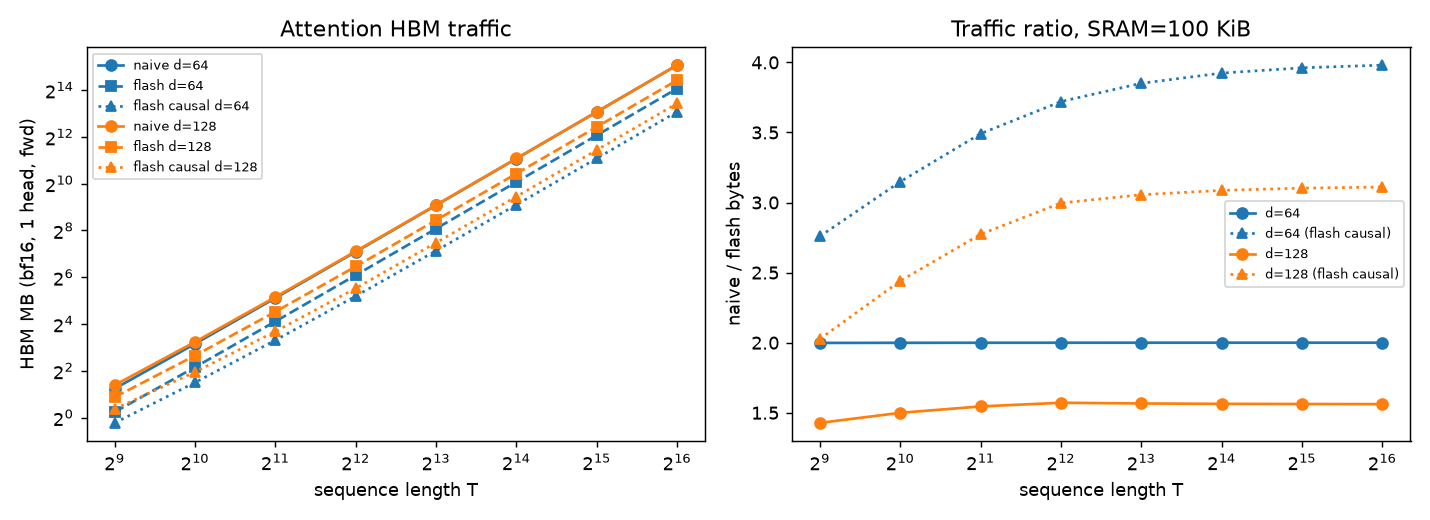
\includegraphics[width=\linewidth]{attention_io.png}
\caption{CPU 部分的 IO 模型（\texttt{attention\_io.csv}）：SRAM=100 KiB、bf16、单头前向。左：朴素与 flash 的 HBM 字节随 $T$ 变化；右：二者之比。}
\label{fig:cpu-io}
\end{figure}

\Cref{fig:cpu-io} 是本文后面要在 GPU 上检验的「理论」。按 FlashAttention 论文的块大小 $B_c=\lfloor M/4d\rfloor$、$B_r=\min(B_c,d)$，$d=64$ 时 $B_r=64$，
K/V 要重读 $T/B_r$ 遍，flash 的流量是 $2T^2d/B_r\approx 2T^2$ 个元素，朴素是 $4T^2$，所以比值固定在 2.00（因果时约 4 倍，$T=65536$ 时 3.98）。
这张图暗示的结论是：FlashAttention 的主要收益不是改变流量的阶，而是把显存从 $O(T^2)$ 降到 $O(T)$。GPU 结果会修正这个结论的后半句：
在真实 GPU 上，朴素实现的流量常数比 4 大（eager 实现是 6 或 8），flash 的块也比 $d$ 大（$B_r=128$），而 L2 又吸收了大部分 K/V 重读。

\begin{figure}[H]
\centering
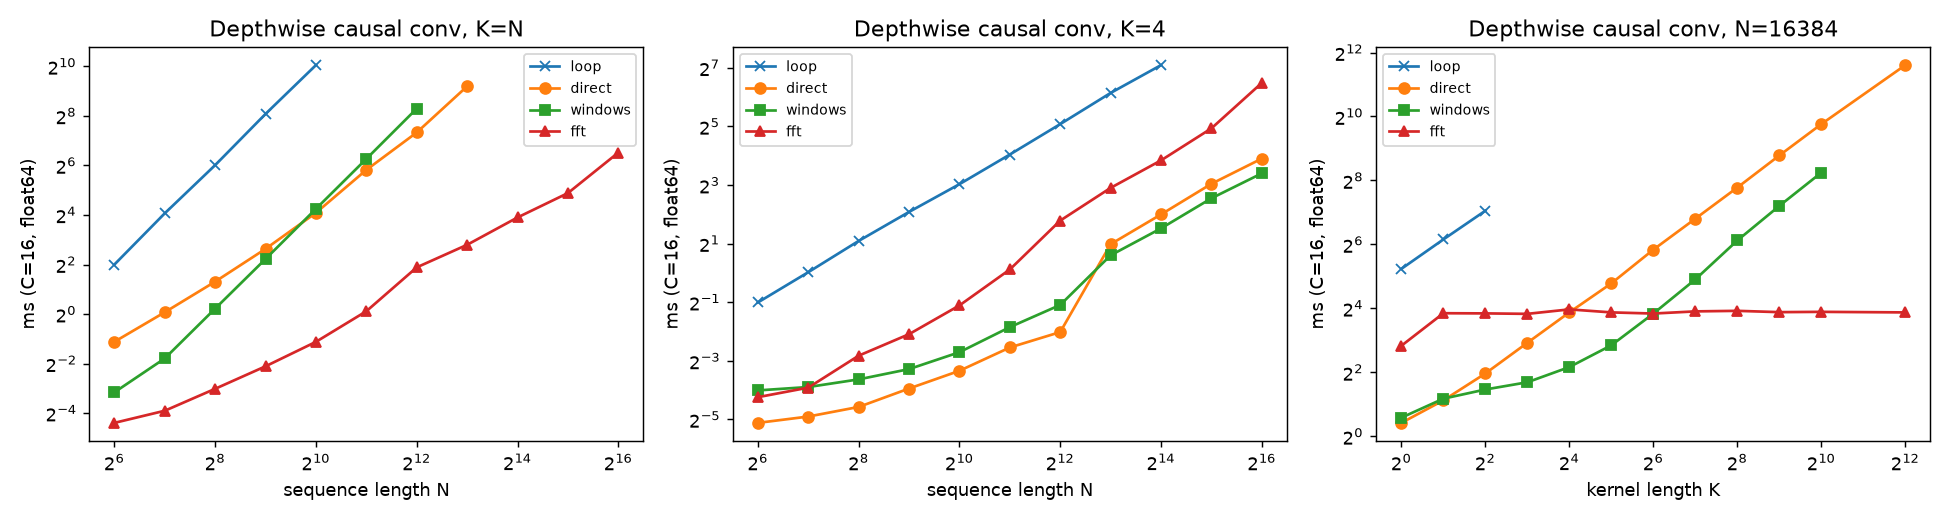
\includegraphics[width=\linewidth]{conv1d_timing.png}
\caption{CPU 部分的 depthwise 因果卷积计时（\texttt{conv1d\_timing.csv}，$C=16$，float64，numpy）。}
\label{fig:cpu-conv}
\end{figure}

\Cref{fig:cpu-conv} 中 FFT 的耗时只取决于 $N$（$N=16384$ 时 14–15 ms），$O(NK)$ 写法随 $K$ 线性增长；CPU 上移位相加在 $K\approx16$、滑窗在 $K\approx64$ 与 FFT 交叉。
GPU 上交叉点会右移到 $K\approx1600$（\cref{sec:conv}）：直接卷积在 GPU 上吃到了 45 TFLOP/s 的算力，而 FFT 是访存受限的。

\begin{figure}[H]
\centering
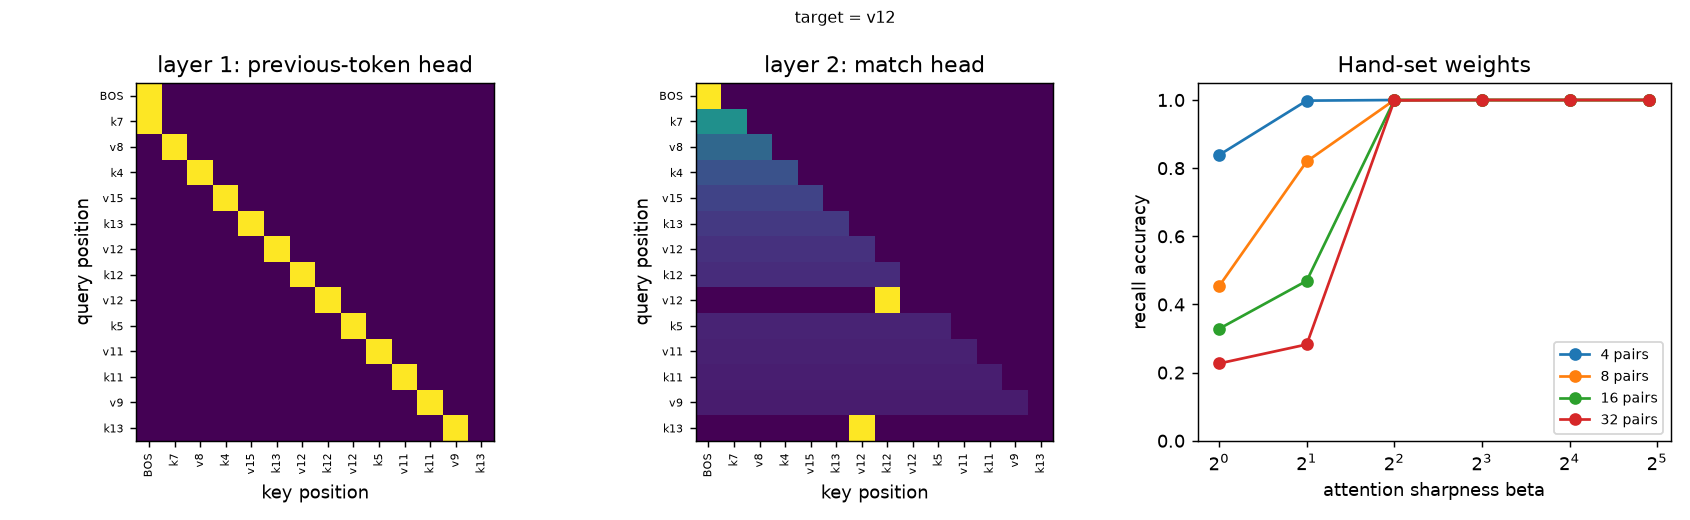
\includegraphics[width=\linewidth]{recall_attention.png}
\caption{手工设定权重的两层 associative recall transformer（\texttt{recall\_accuracy.csv}）。左、中：两层的注意力图；右：准确率随注意力锐度 $\beta$ 的变化。}
\label{fig:cpu-recall}
\end{figure}

\Cref{fig:cpu-recall}：第 1 层 query $=\beta\,e_{\text{pos}}(p)$、key $=e_{\text{pos}}(j+1)$，于是位置 $p$ 注意到 $p-1$，把 $\text{tok}(p-1)$ 写进 prev 子空间；
第 2 层 query $=\beta\,\text{tok}(p)$、key $=\text{prev}(j)$，最后一个位置（查询键 $q$）注意到「前一个 token 是 $q$」的位置，即对应的 value。
$\beta\ge8$ 时 4–32 对键值都是 100\% 准确；$\beta=1$ 时 32 对只有 0.2268。这正是 induction head\cite{induction} 的两步结构，后面的 MQAR 训练会说明 1 层模型学不出它（\cref{sec:train}）。

\subsection{FlashAttention 前向：时间、吞吐、显存与误差}\label{sec:flash}

\begin{figure}[H]
\centering
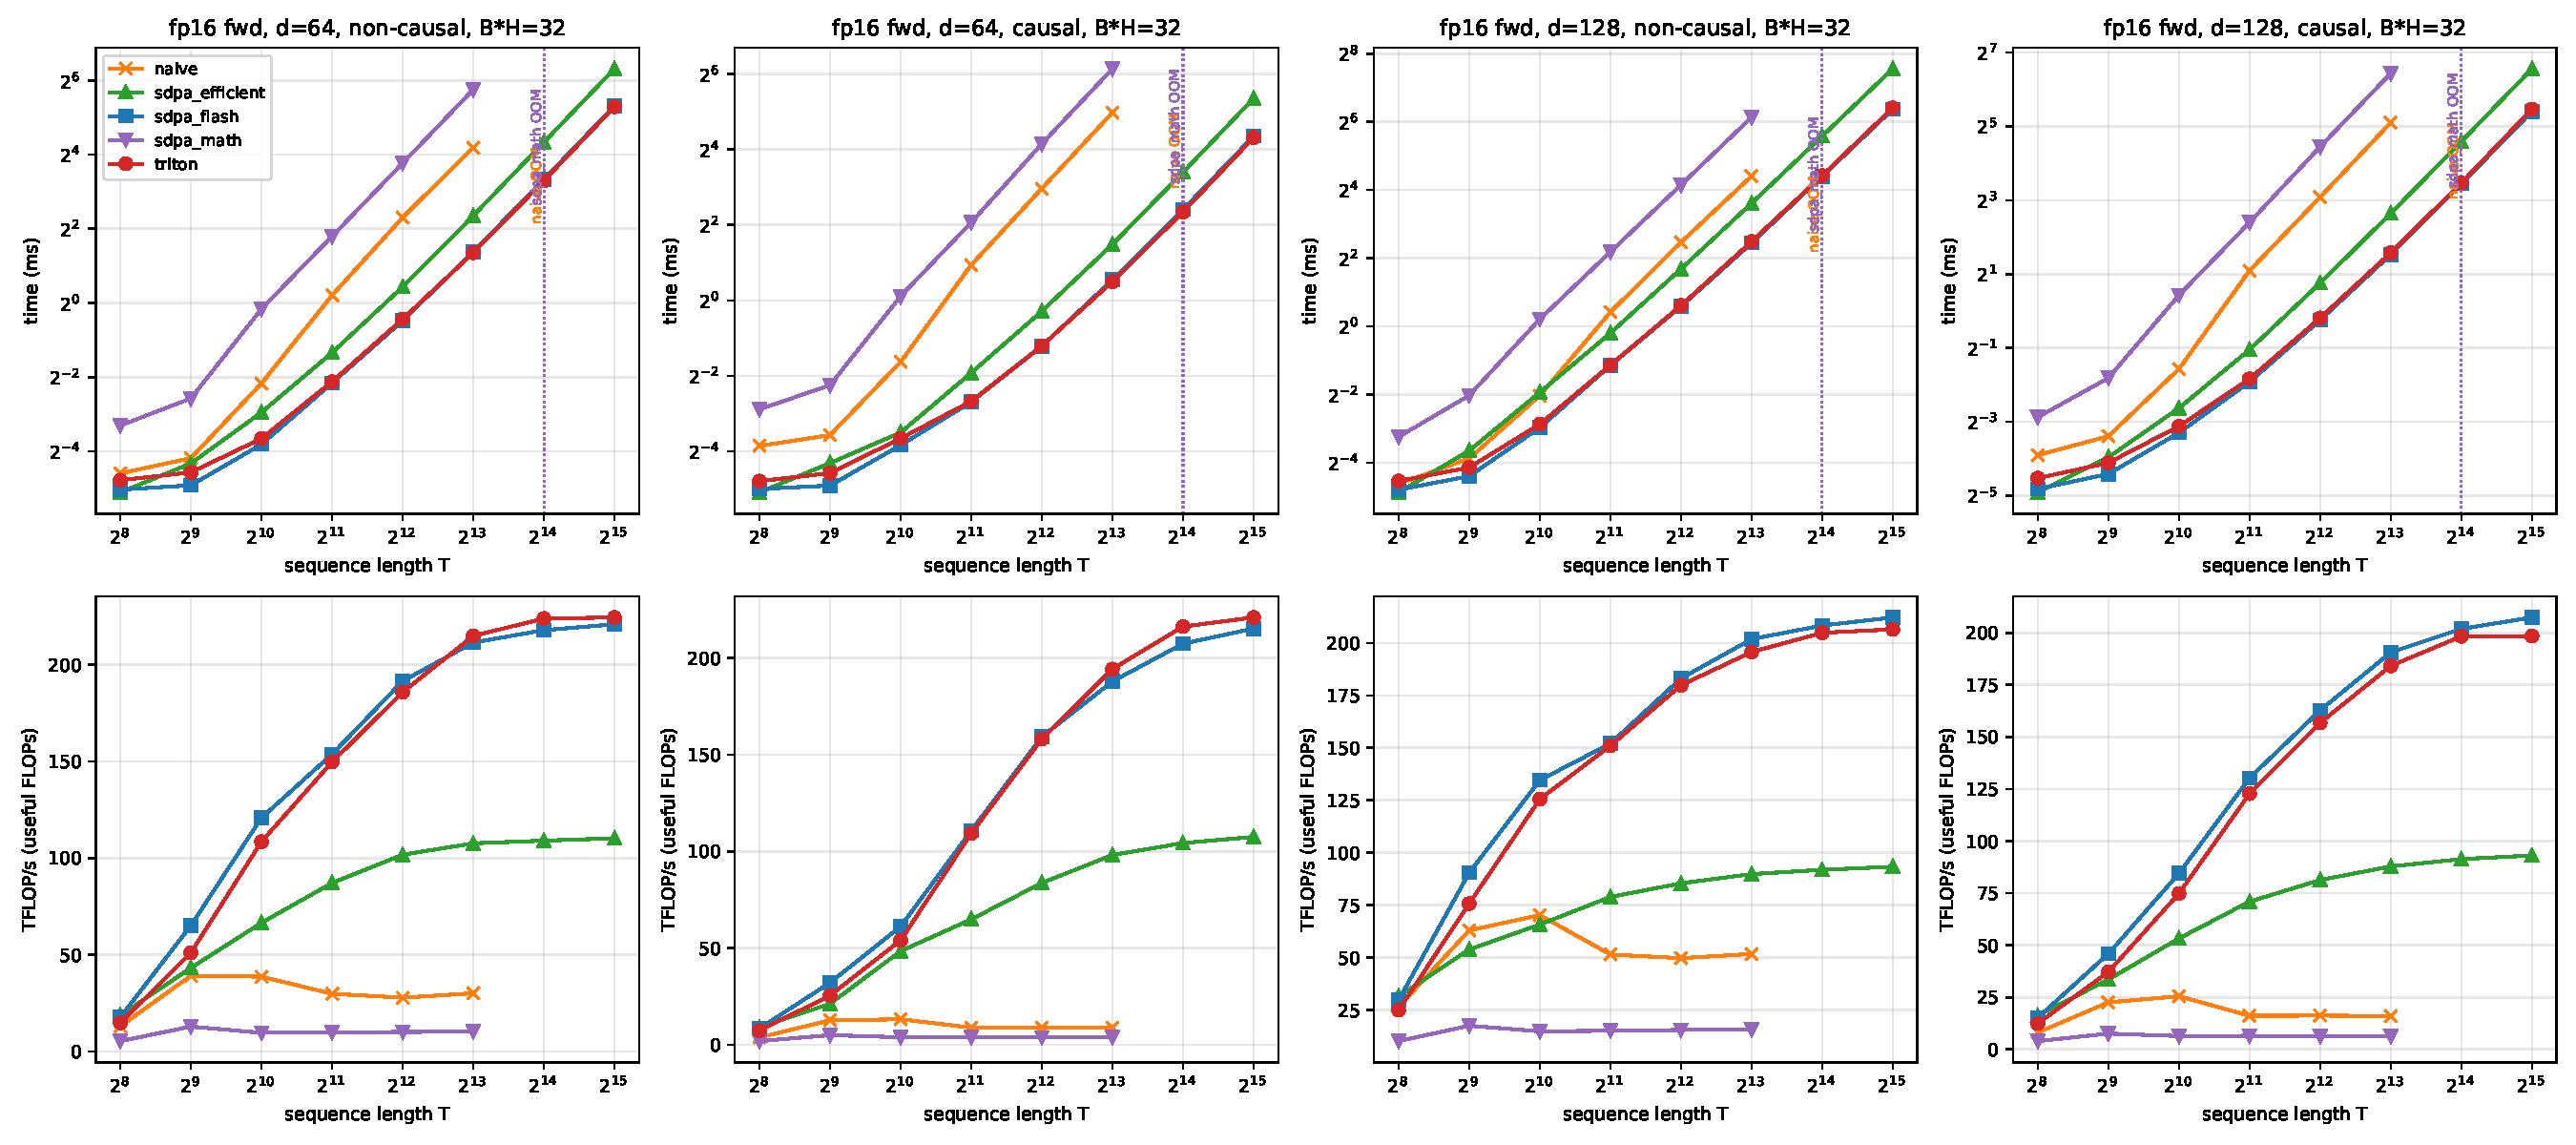
\includegraphics[width=\linewidth]{gpu_attn_fwd_time_tflops.pdf}
\caption{fp16 前向，$B=2,H=16$。上：时间（log-log），竖虚线是 OOM 点；下：有用 FLOPs 的吞吐（\texttt{attention\_fwd.jsonl}）。}
\label{fig:fwd}
\end{figure}

\begin{table}[H]
\centering\small
\caption{fp16 前向，$d=64$，非因果，$B\cdot H=32$（ms / TFLOP/s；「额外显存」为输入之外的峰值）}\label{tab:fwd}
\begin{tabular}{lrrrrr}
\toprule
方法 & $T=1024$ & $T=4096$ & $T=8192$ & $T=16384$ & $T=32768$ \\
\midrule
Triton（本文） & 0.079 / 108.5 & 0.739 / 185.9 & 2.558 / 214.9 & 9.818 / 224.0 & 39.18 / 224.5 \\
SDPA flash & 0.071 / 120.9 & 0.717 / 191.6 & 2.599 / 211.5 & 10.09 / 217.9 & 39.81 / 221.0 \\
SDPA efficient & 0.129 / 66.5 & 1.350 / 101.8 & 5.107 / 107.6 & 20.17 / 109.0 & 79.78 / 110.2 \\
SDPA math & 0.894 / 9.6 & 13.66 / 10.1 & 54.06 / 10.2 & OOM & — \\
朴素 PyTorch & 0.222 / 38.7 & 4.943 / 27.8 & 18.28 / 30.1 & OOM & — \\
\midrule
额外显存：Triton & 4.3 MB & 17.3 MB & 34.6 MB & 69.2 MB & 138.4 MB \\
额外显存：朴素 & 138 MB & 2.16 GB & 8.62 GB & OOM & — \\
\bottomrule
\end{tabular}
\end{table}

\Cref{fig:fwd,tab:fwd} 说明四件事。
第一，本文的 Triton kernel 与 PyTorch 自带的 FlashAttention-2 基本持平：$T\ge8192$ 时略快（$d=64$ 非因果 $T=16384$：224.0 对 217.9 TFLOP/s；因果 216.2 对 207.4），
$T\le2048$ 时略慢（$T=1024$：108.5 对 120.9），$d=128$ 时慢 2–4\%（$T=32768$ 因果 198.4 对 207.4）。短序列的差距来自启动与尾部效应：$T=1024$、$B_r=128$ 时只有 $8\times32=256$ 个 program，每个 SM 平均 1.5 个，波次量化损失明显。
第二，峰值 224.5 TFLOP/s 是实测 BF16 方阵乘峰值（236.3）的 95\%，attention 已经是计算受限。
第三，朴素实现的吞吐随 $T$ 下降并停在 28–30 TFLOP/s（$d=64$），因果时只有 8.7 TFLOP/s：它是访存受限的（\cref{sec:theory} 会把这个数解释到 93\%）。$T=8192$ 时 Triton 比朴素快 7.15 倍（非因果）和 22.2 倍（因果，31.47 对 1.415 ms）。
第四，SDPA 的 math 后端比朴素实现还慢 3 倍（$T=4096$：13.66 对 4.94 ms），额外显存是朴素的 2.3 倍（4.97 对 2.16 GB）：它在 fp16 输入下仍按通用路径做了更多中间张量。

\begin{figure}[H]
\centering
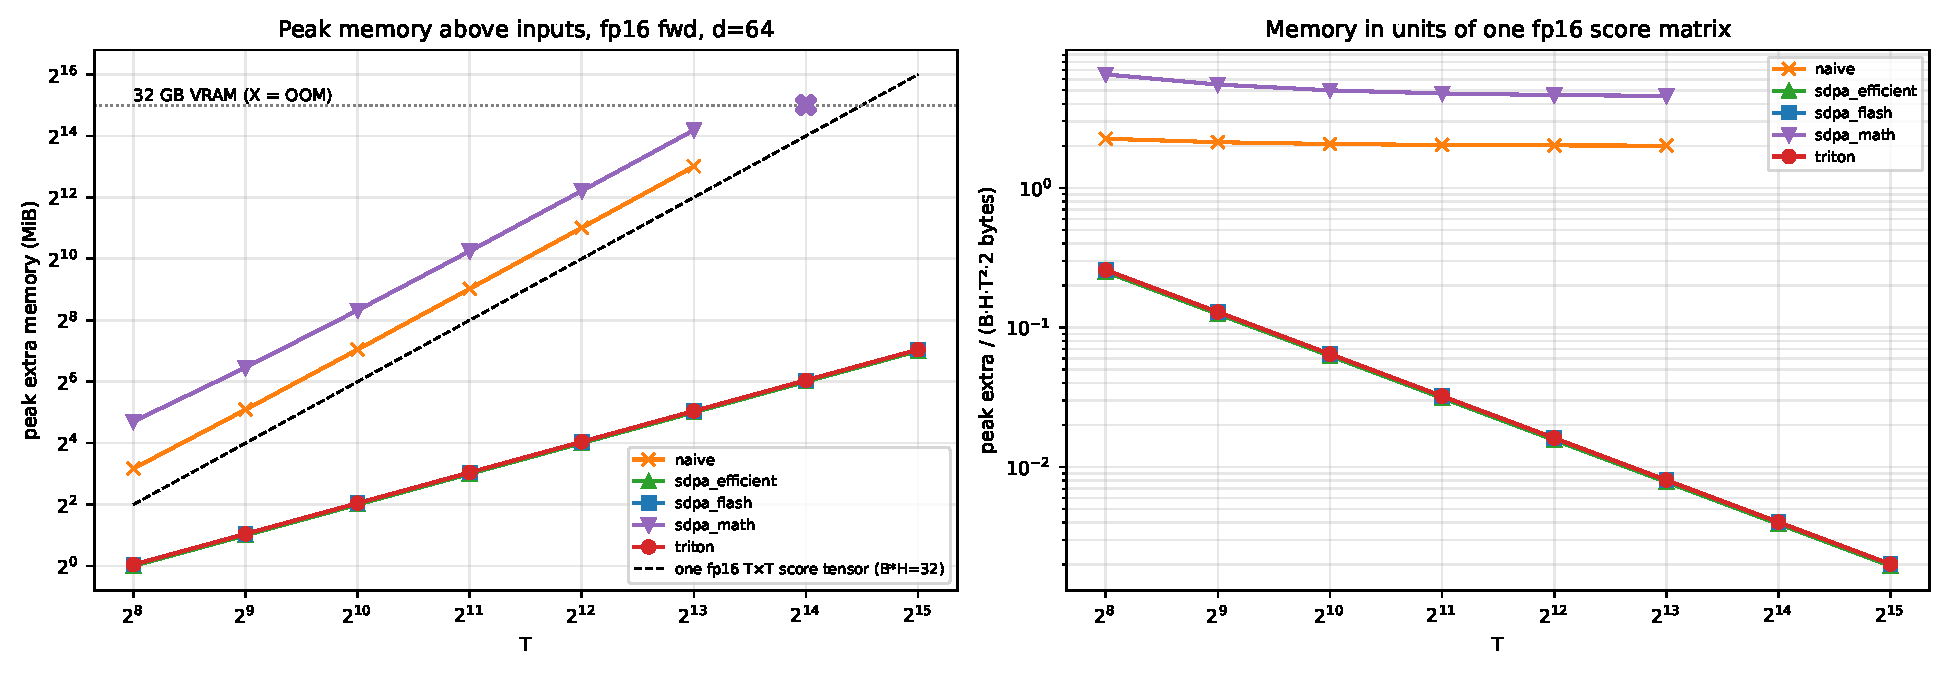
\includegraphics[width=\linewidth]{gpu_attn_peak_memory.pdf}
\caption{峰值额外显存（fp16，$d=64$，非因果）。左：绝对值，虚线是一个 fp16 $T\times T$ 分数张量；右：以一个分数张量为单位。}
\label{fig:mem}
\end{figure}

\Cref{fig:mem} 是 FlashAttention 最直接的收益。朴素实现的峰值恰好是 2 个 fp16 分数矩阵（$T=8192$：8.62 GB $=2\times32\times8192^2\times2$ B），
对应 matmul 写出的 $S$ 和 softmax 写出的 $P$ 同时存活（中间的 \texttt{*scale} 产生的临时张量在下一步就被释放）；math 后端是 4 个以上。
因此 32 GB 的卡在 $B\cdot H=32$ 时，$T=16384$ 的两个分数矩阵需要 34.4 GB，必然 OOM——这正是记录到的 OOM 点。
flash 类方法的额外显存只有输出 $O$ 加 lse：$32\times T\times(64\times2+4)$ 字节，$T=32768$ 时 138.4 MB，与 $T$ 线性，右图的斜率是 $-1$。

\begin{figure}[H]
\centering
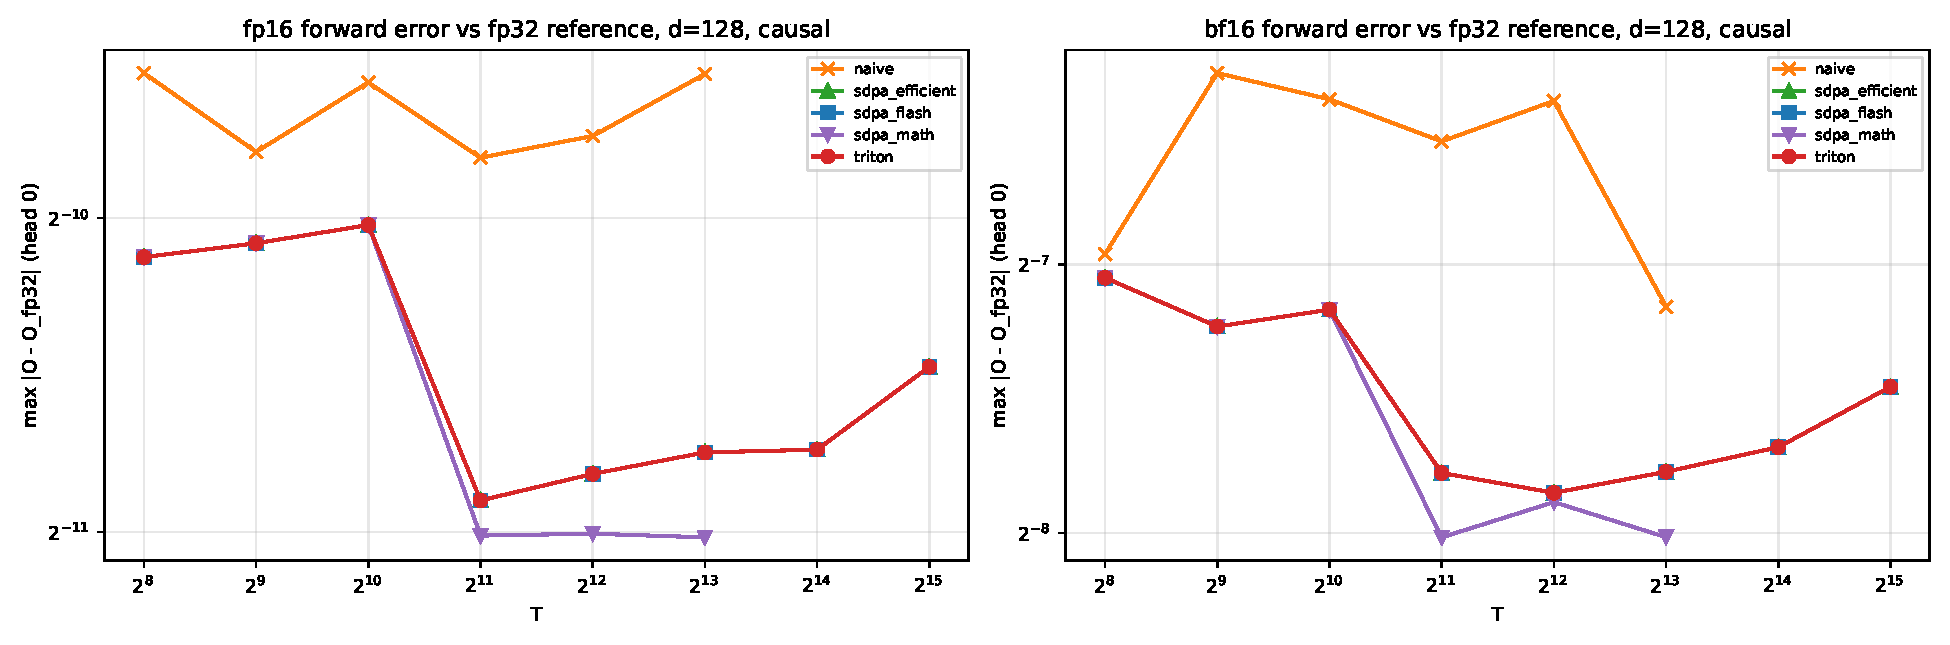
\includegraphics[width=\linewidth]{gpu_attn_error.pdf}
\caption{与 fp32 参考的最大绝对误差（head 0，$d=128$，因果）。左 fp16，右 bf16。}
\label{fig:err}
\end{figure}

\Cref{fig:err}：所有 flash 类实现（Triton、SDPA flash/efficient）的误差几乎相同，因为它们都在 fp32 中累加、只在 $P\cdot V$ 前把 $P$ 舍入为 16 位。
fp16 下 $T=4096$ 非因果 $d=64$ 的最大误差是 6.6e-5，bf16 是 3.65e-4，比值约 5.5，接近两种格式尾数精度之比（$2^{-11}$ 对 $2^{-8}$ 是 8 倍）。
朴素实现误差大 2–4 倍（fp16 1.43e-4），因为它把 $S$ 也以 fp16 写回显存、再做 softmax。因果时误差反而更大（fp16 约 5e-4–9e-4），而且不随 $T$ 下降：
因果序列的前几行只对很少几个 value 取平均，舍入误差没有被平均掉；非因果时误差随 $T$ 下降（$T=32768$ 时 2.2e-5），因为输出是对更多 value 的平均，幅值本身变小。

\subsection{反向}\label{sec:bwd}

\begin{figure}[H]
\centering
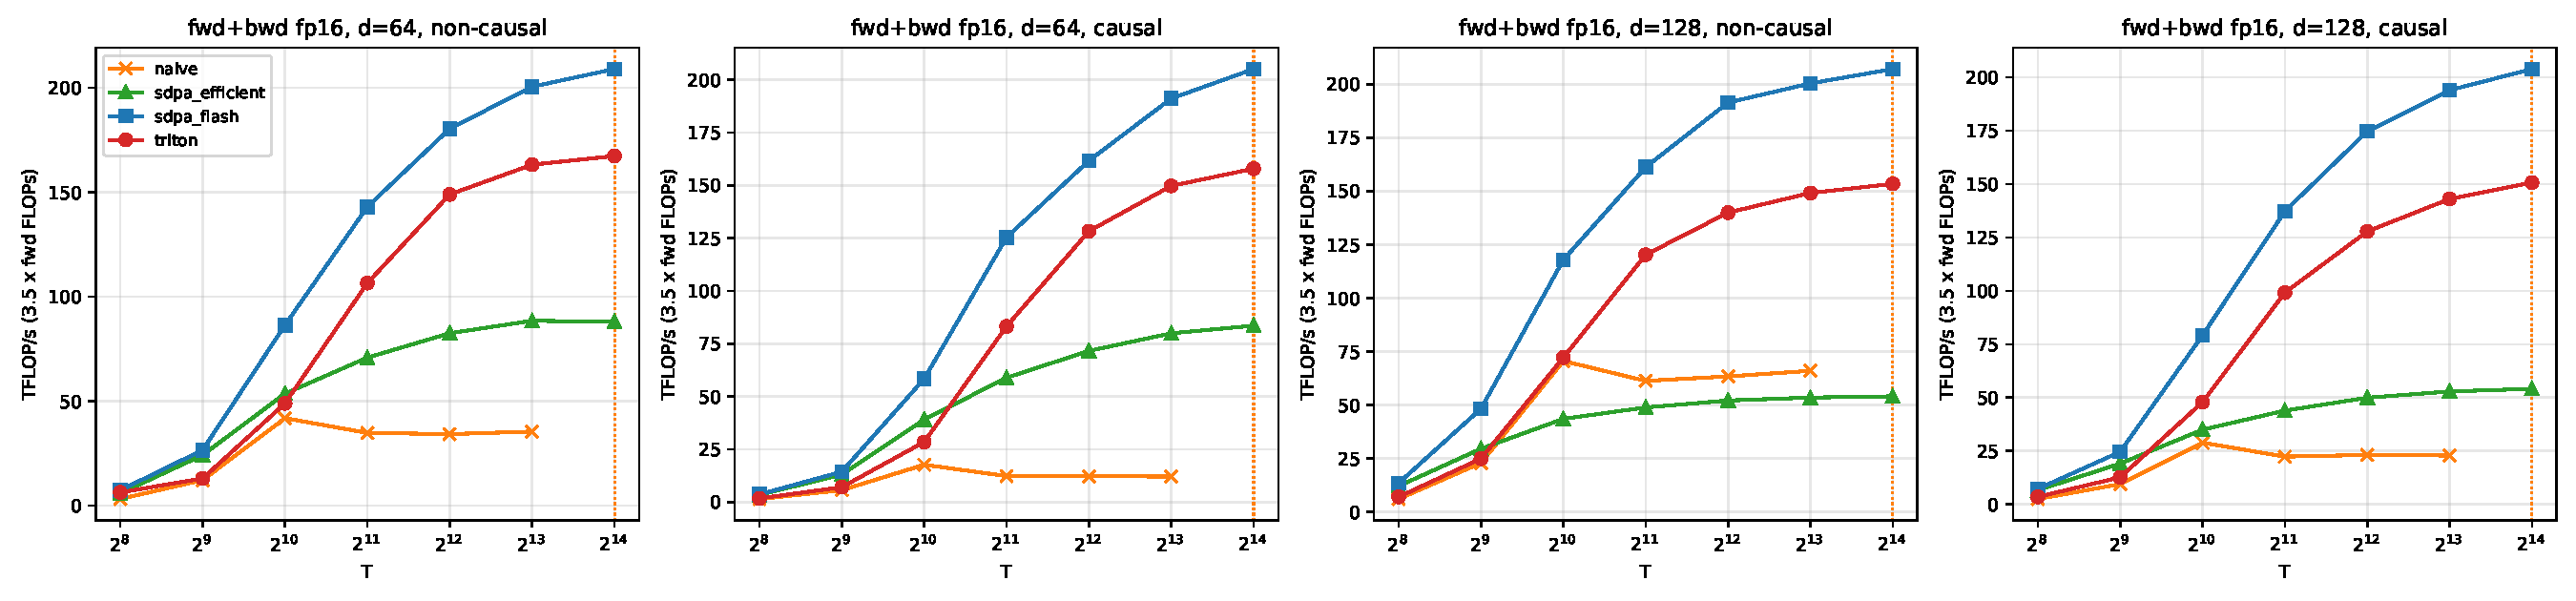
\includegraphics[width=\linewidth]{gpu_attn_fwd_bwd.pdf}
\caption{前向 + 反向吞吐（fp16，$B\cdot H=32$，FLOPs 记为前向的 3.5 倍；\texttt{attention\_bwd.jsonl}）。}
\label{fig:bwd}
\end{figure}

\Cref{fig:bwd}：Triton 反向的梯度误差与 SDPA flash 一致（$T=4096$、$d=64$ 非因果，$dQ$ 最大误差都是 8.8e-5），所以实现是正确的；
但速度是 SDPA flash 的 80\%：$d=64$ 非因果 $T=16384$ 时 45.99 对 36.83 ms（167.4 对 209.0 TFLOP/s），$d=128$ 时 153.4 对 207.1 TFLOP/s。
原因在 \cref{sec:impl-bwd}：两个独立 kernel 各自重算 $QK^\top$ 与 $dO\,V^\top$，反向的矩阵乘是 7 个而不是 5 个；计入前向的 2 个，总量是 9 对 7，
若每个矩阵乘效率相同，上限就是 $7/9=78\%$——实测 80\% 说明单个矩阵乘的效率与 FA2 相当，差距几乎全部来自多余的计算。
短序列时 Triton 有约 0.53 ms 的平台（$T=256$ 到 $1024$ 几乎不变），这是主机侧开销：autograd、PyTorch 计算 $D$、两个 Triton launcher 在只有 2 个 CPU 核的环境下各需几十微秒。
朴素实现 $T=8192$ 时峰值 17.1 GB（要为反向保存 $P$），$T=16384$ OOM；efficient 后端在 $d=128$ 时只有 54 TFLOP/s。

\subsection{batch$\times$heads 与占用率}\label{sec:bh}

\begin{figure}[H]
\centering
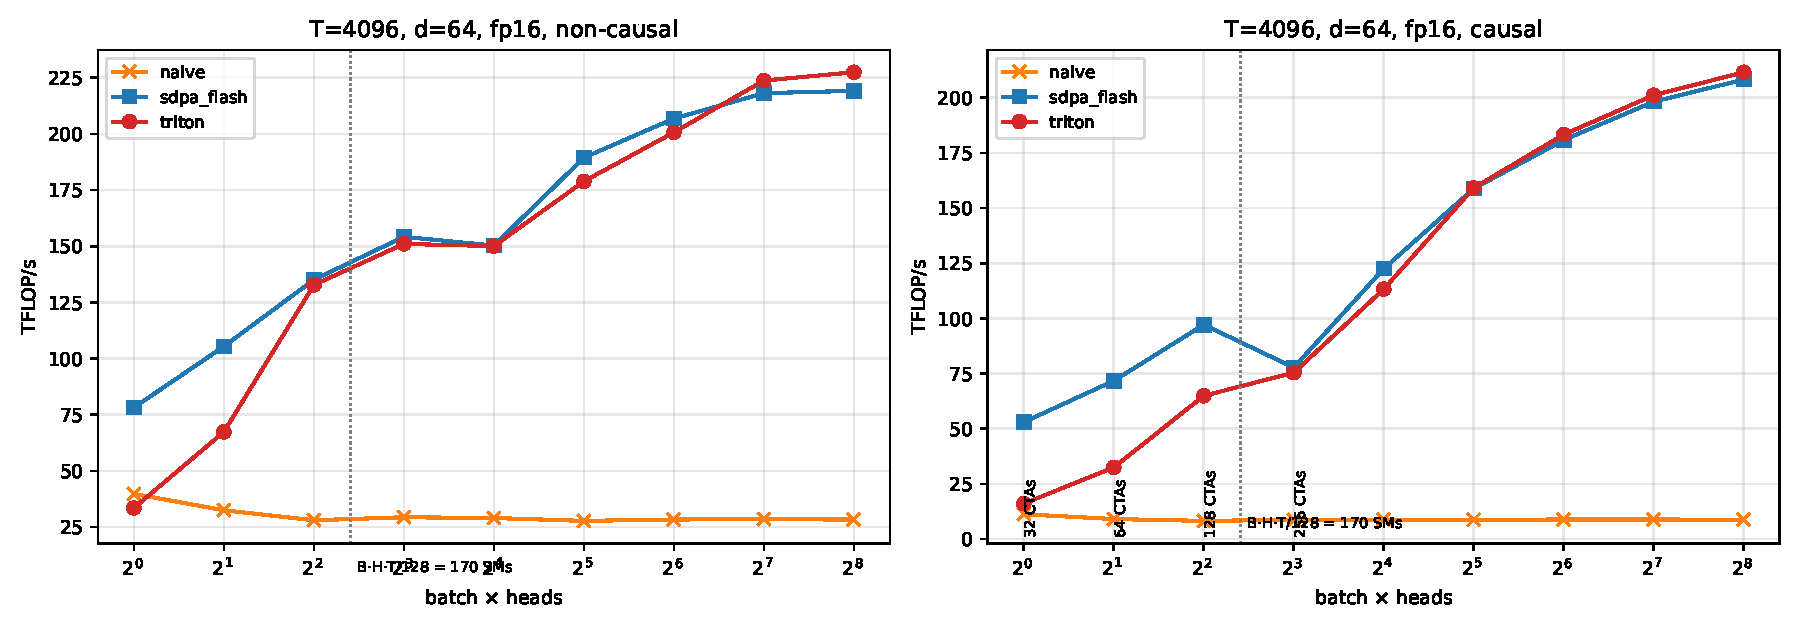
\includegraphics[width=\linewidth]{gpu_attn_batch_heads.pdf}
\caption{$T=4096$、$d=64$ 时吞吐随 $B\cdot H$ 的变化（\texttt{attention\_bh.jsonl}）。标注为 Triton 默认块下的 program 数。}
\label{fig:bh}
\end{figure}

\Cref{fig:bh}：网格大小是 $\lceil T/B_r\rceil\times BH$。$BH=1$ 时只有 32 个 program，而 GPU 有 170 个 SM，Triton 只有 33.5 TFLOP/s；
SDPA flash 在同样形状下有 78.2 TFLOP/s，说明它对小网格用了更小的块或 split 策略。$BH\ge4$（128 个 program）后两者几乎重合，
$BH=256$ 时 Triton 227.4、SDPA flash 219.2 TFLOP/s。因果时小网格的劣势更明显（$BH=1$：16.1 对 53.0），因为各 Q 块工作量不同，最重的那个 program 决定总时间。
这条曲线是 decode 阶段要用 split-K（Flash-Decoding\cite{flashdecoding}）的原因：decode 时每个序列只有 1 行 query，网格天然太小。

\subsection{块大小扫描与 IO 模型}\label{sec:blocks}

\begin{figure}[H]
\centering
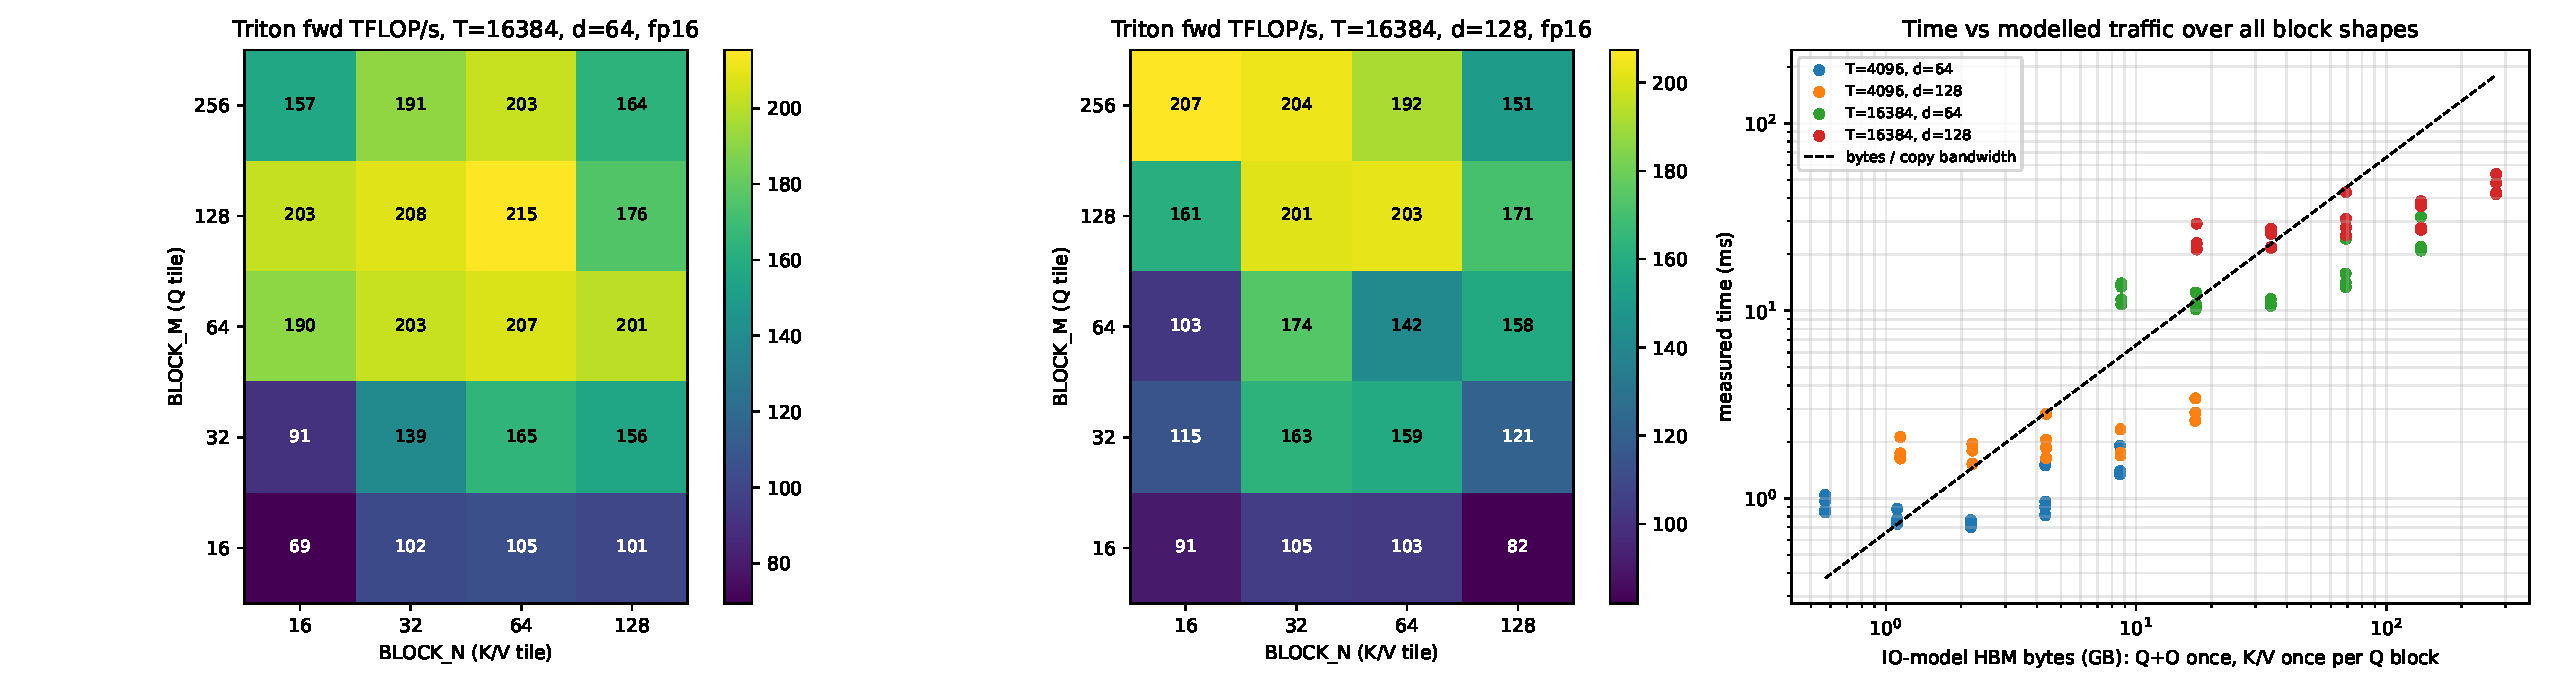
\includegraphics[width=\linewidth]{gpu_attn_block_sweep.pdf}
\caption{Triton 前向的 $B_r\times B_c$ 扫描（fp16，非因果，$B\cdot H=32$，\texttt{attention\_blocks.jsonl}）。左、中：$T=16384$ 的 TFLOP/s；右：所有块形状的实测时间对 IO 模型字节，虚线是「字节 ÷ copy 带宽」。}
\label{fig:blocks}
\end{figure}

IO 模型（与 CPU 部分 \texttt{flash\_elements} 相同的计数方式）：$Q$ 和 $O$ 各读写一次，每个 Q 块把整段 K/V 读一遍，
\begin{equation}
\text{bytes}_{\text{flash}} = BH\left[2\,(2Td + \lceil T/B_r\rceil\cdot 2Td) + 4T\right].\label{eq:flashbytes}
\end{equation}
\Cref{fig:blocks} 左、中两图：$d=64$ 时最佳块是 $(B_r,B_c)=(128,64)$，215.4 TFLOP/s；$d=128$ 时 $(256,16)$ 207.4 与 $(128,64)$ 202.8 接近。
$B_r=16$ 时吞吐只有一半（$d=64$：105.0），$B_r=256$ 时又下降（203.2），$B_c=128$ 普遍差（寄存器溢出或共享内存只能单级流水）。

右图是本节的关键：如果 \cref{eq:flashbytes} 就是 DRAM 流量，那么所有点都应该在虚线（1.52 TB/s）上方。
实际上 $B_r=16$ 的点全在虚线下方很远：$T=16384$、$d=64$、$(16,64)$ 的模型字节是 137.6 GB，耗时 20.94 ms，隐含带宽 6.57 TB/s，是 DRAM 带宽的 4.3 倍。
唯一的解释是大部分 K/V 重读命中了 L2：同一个 head 的 K/V 只有 $2\times16384\times64\times2=4$ MB，并发运行的几百个 program 里同一 head 的 Q 块共享这 4 MB，96 MB 的 L2 能放下 24 个 head 的 K/V。
所以教科书 IO 模型对 GPU 是 DRAM 流量的\textbf{上界}，GPU 上真正决定 $B_r$ 的不是 DRAM 流量，而是 tensor core 的利用率与寄存器压力。

\begin{figure}[H]
\centering
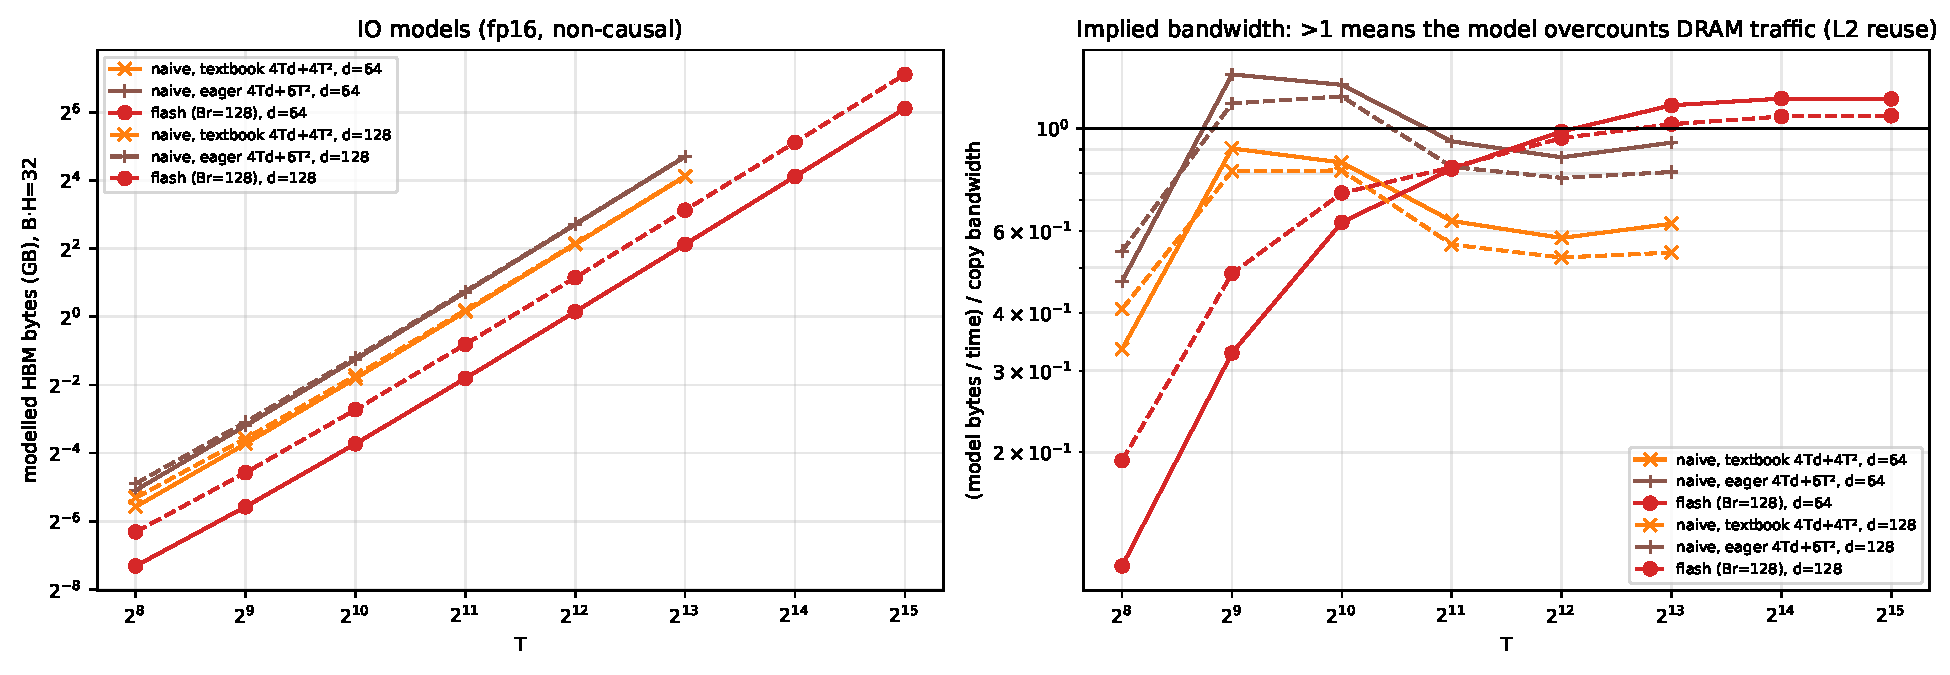
\includegraphics[width=\linewidth]{gpu_attn_io_model.pdf}
\caption{左：三种字节模型（fp16，非因果，$B\cdot H=32$）；右：模型字节 ÷ 实测时间 ÷ copy 带宽。大于 1 表示模型高估了 DRAM 流量。}
\label{fig:io}
\end{figure}

\Cref{fig:io} 把 CPU 部分的 IO 模型直接放到 GPU 时间上对照：
\begin{itemize}
\item 朴素实现按教科书 $4Td+4T^2$ 计算，$T\ge2048$ 时隐含带宽只有 copy 带宽的 0.55–0.62；按 eager 实际的 $4Td+6T^2$（多了 \texttt{*scale} 的一读一写）计算，$d=64$、$T=8192$ 时为 25.90 GB ÷ 18.28 ms = 1.417 TB/s，是 copy 带宽的 93\%。朴素实现就是一个以 DRAM 带宽运行的访存程序。
  $T=512$–$1024$ 时 eager 曲线超过 1，因为整个分数张量（$T=1024$ 时 $32\times1024^2\times2=67$ MB）放得进 96 MB L2，读写不必到 DRAM。
\item Triton（$B_r=128$）$T\ge4096$ 时比值超过 1（$T=16384$：17.31 GB ÷ 9.818 ms = 1.76 TB/s，1.16 倍），同样说明 L2 吸收了至少 14\% 的 K/V 重读。
\item 字节比与时间比不同：模型给出朴素/flash 的字节比约 $2B_r/d\cdot\frac{6}{4}=6$（$d=64$），实测时间比 7.15；flash 是计算受限的，时间比本来就不该等于字节比。
\end{itemize}

\subsection{Roofline：一层 Llama-2-7B 的 prefill 与 decode}\label{sec:roof}

\begin{figure}[H]
\centering
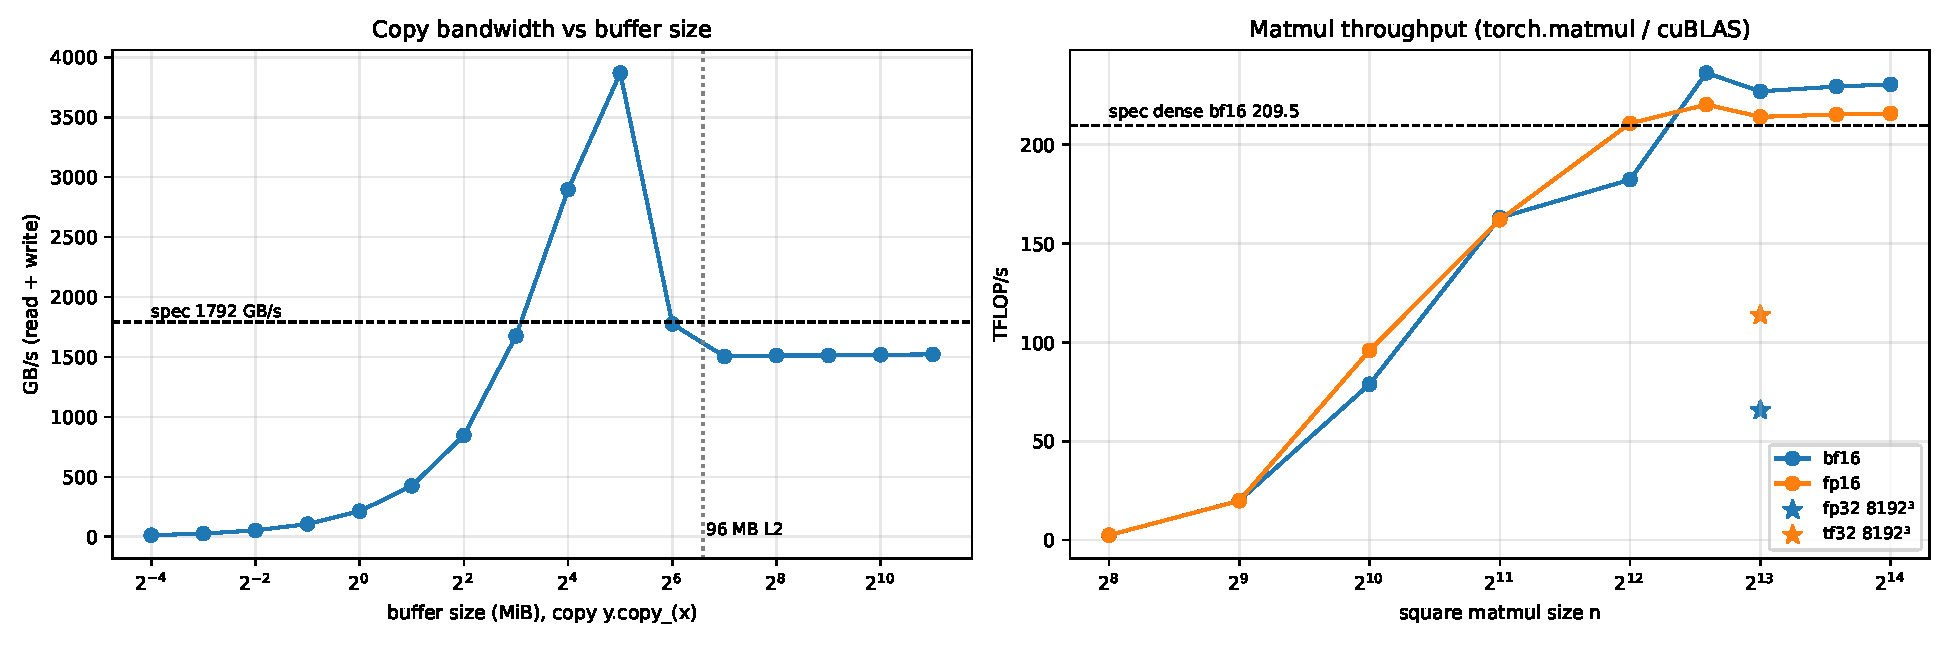
\includegraphics[width=\linewidth]{gpu_peak_bw_flops.pdf}
\caption{左：copy 带宽随缓冲大小（32 MiB 处 3.87 TB/s 是 L2 带宽，$\ge128$ MiB 收敛到 1.50–1.52 TB/s）；右：方阵乘吞吐（\texttt{roofline.jsonl}）。}
\label{fig:peaks}
\end{figure}

\Cref{fig:peaks} 给出 roofline 的两个参数。copy 带宽在缓冲 $\le32$ MiB（两个缓冲共 64 MiB，放得进 96 MB L2）时达到 3869 GB/s，
64 MiB 时开始掉，$\ge128$ MiB 时稳定在 1504–1522 GB/s，是规格 1792 GB/s 的 85\%；只读求和是 1626 GB/s。
矩阵乘在 $n\le1024$ 时受启动开销限制（$n=256$ 只有 2.5 TFLOP/s，单次 13.5 µs），$n=6144$ 达到峰值 236.3 TFLOP/s；
fp16（fp32 累加）稍低，为 220.3；fp32 不用张量核只有 65.7，TF32 113.8。

\begin{figure}[H]
\centering
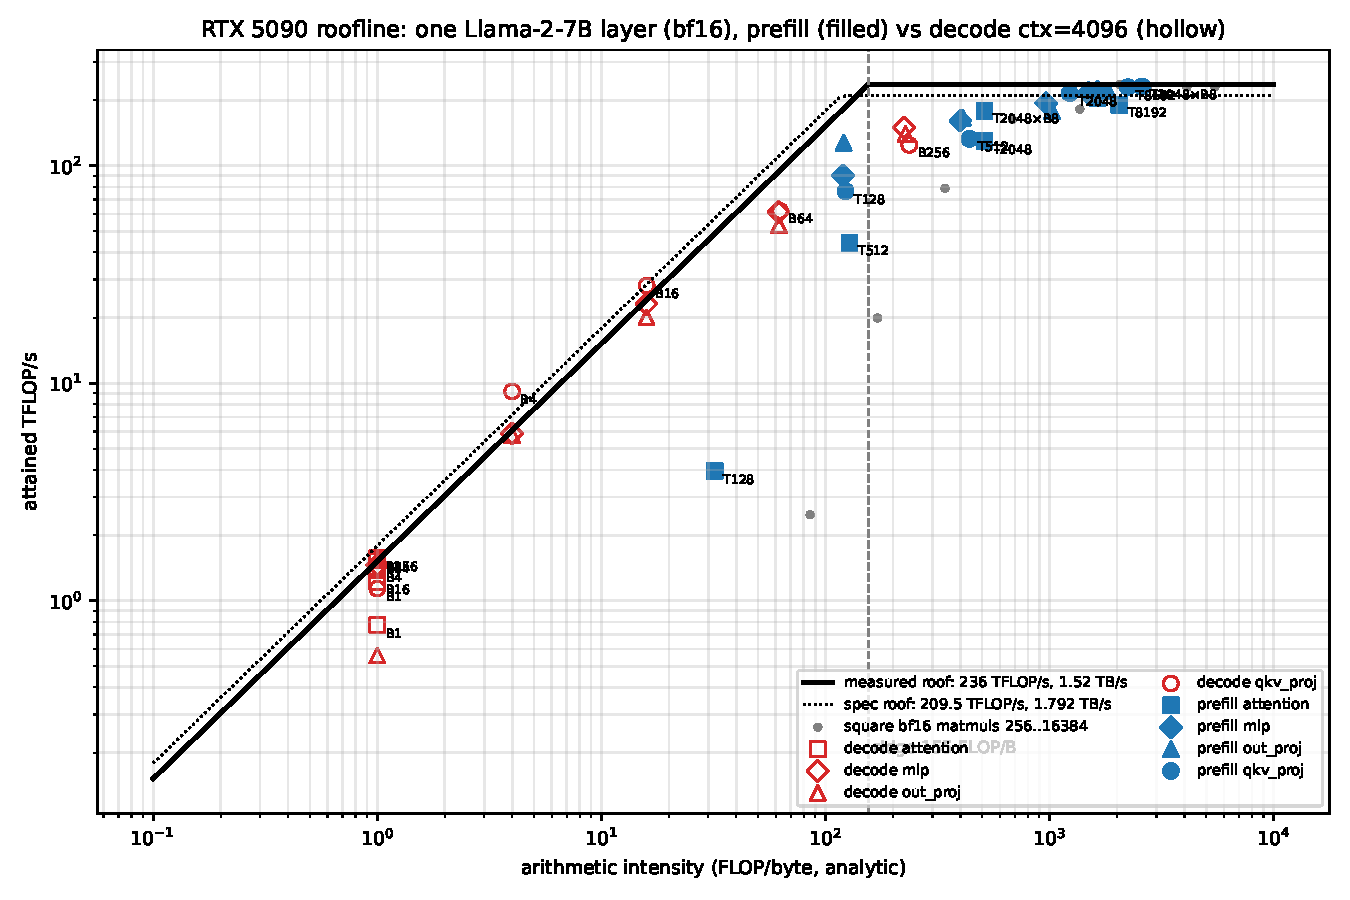
\includegraphics[width=\linewidth]{gpu_roofline_layer.pdf}
\caption{RTX 5090 roofline。横坐标为 \texttt{mlsys\_calc} 的解析强度，纵坐标为实测吞吐；实心为 prefill，空心为 decode（上下文 4096）。}
\label{fig:roof}
\end{figure}

\begin{table}[H]
\centering\small
\caption{一层 Llama-2-7B 各算子（bf16；eff = roofline 时间 ÷ 实测时间，roofline 用实测峰值）}\label{tab:roof}
\begin{tabular}{llrrrrr}
\toprule
形状 & 算子 & 强度 (FLOP/B) & ms & TFLOP/s & GB/s & eff \\
\midrule
decode $B=1$ & QKV 投影 & 1.00 & 0.0884 & 1.14 & 1139 & 0.75 \\
 & attention & 1.00 & 0.0868 & 0.77 & 773 & 0.51 \\
 & MLP & 1.00 & 0.1851 & 1.46 & 1463 & 0.96 \\
decode $B=64$ & QKV 投影 & 62.7 & 0.1039 & 62.0 & 989 & 0.65 \\
 & attention & 1.00 & 2.806 & 1.53 & 1531 & 1.01 \\
decode $B=256$ & QKV 投影 & 236.3 & 0.2067 & 124.7 & 528 & 0.53 \\
 & attention & 1.00 & 10.95 & 1.57 & 1570 & 1.03 \\
prefill $T=128$ & attention & 32 & 0.0341 & 3.94 & 123 & 0.08 \\
prefill $T=8192$ & QKV 投影 & 2234 & 3.589 & 229.8 & 103 & 0.97 \\
 & attention & 2048 & 2.887 & 190.5 & 93 & 0.81 \\
 & MLP & 1491 & 10.27 & 215.8 & 145 & 0.91 \\
\bottomrule
\end{tabular}
\end{table}

\Cref{fig:roof,tab:roof} 是第 3 部分「MHA 算术强度」的实测答案。
\textbf{decode 的 attention 强度恒为 1 FLOP/B}，与 batch 无关：每个序列有自己的 KV cache，加大 batch 只是线性增加要读的字节。
这与 CPU 部分 \texttt{decode\_attention\_intensity} 的公式 $I=2(H/H_{kv})/b$（MHA、$b=2$ 时为 1）完全一致。$B\ge64$ 时它跑到 1.53–1.57 TB/s，
略高于 copy 带宽（因为 attention 几乎只读，只读带宽是 1.63 TB/s）。\textbf{decode 的投影与 MLP 强度约等于 $B$}：$I\approx \frac{2BNK}{2NK}=B$（权重字节占主导），
$B=1$ 时 MLP 读 270 MB 权重达到 1463 GB/s（eff 0.96），$B=256$ 时 QKV 投影强度 236 已越过 ridge（155），变成计算受限，但只达到 124.7 TFLOP/s（$M=256$ 的瘦矩阵乘 tile 利用率差）。
\textbf{prefill 的四个算子都在 ridge 右侧}，$T=8192$ 时 QKV 投影达到 229.8 TFLOP/s（eff 0.97）。$T=128$ 的 attention 只有 3.94 TFLOP/s（eff 0.08），这是一个 34 µs 的 kernel，几乎全是启动开销。

一个细节：decode $B=4$ 的 QKV 投影 eff 为 1.51，超过 1。它的权重是 $4096\times12288\times2=100.7$ MB，与 96 MB L2 相当，重复测量时有一部分权重留在 L2 中。
真实推理中各层权重轮流使用，不会有这种 L2 命中，所以小 batch 的投影应按 eff $\approx0.75$–$0.96$ 理解。

\begin{figure}[H]
\centering
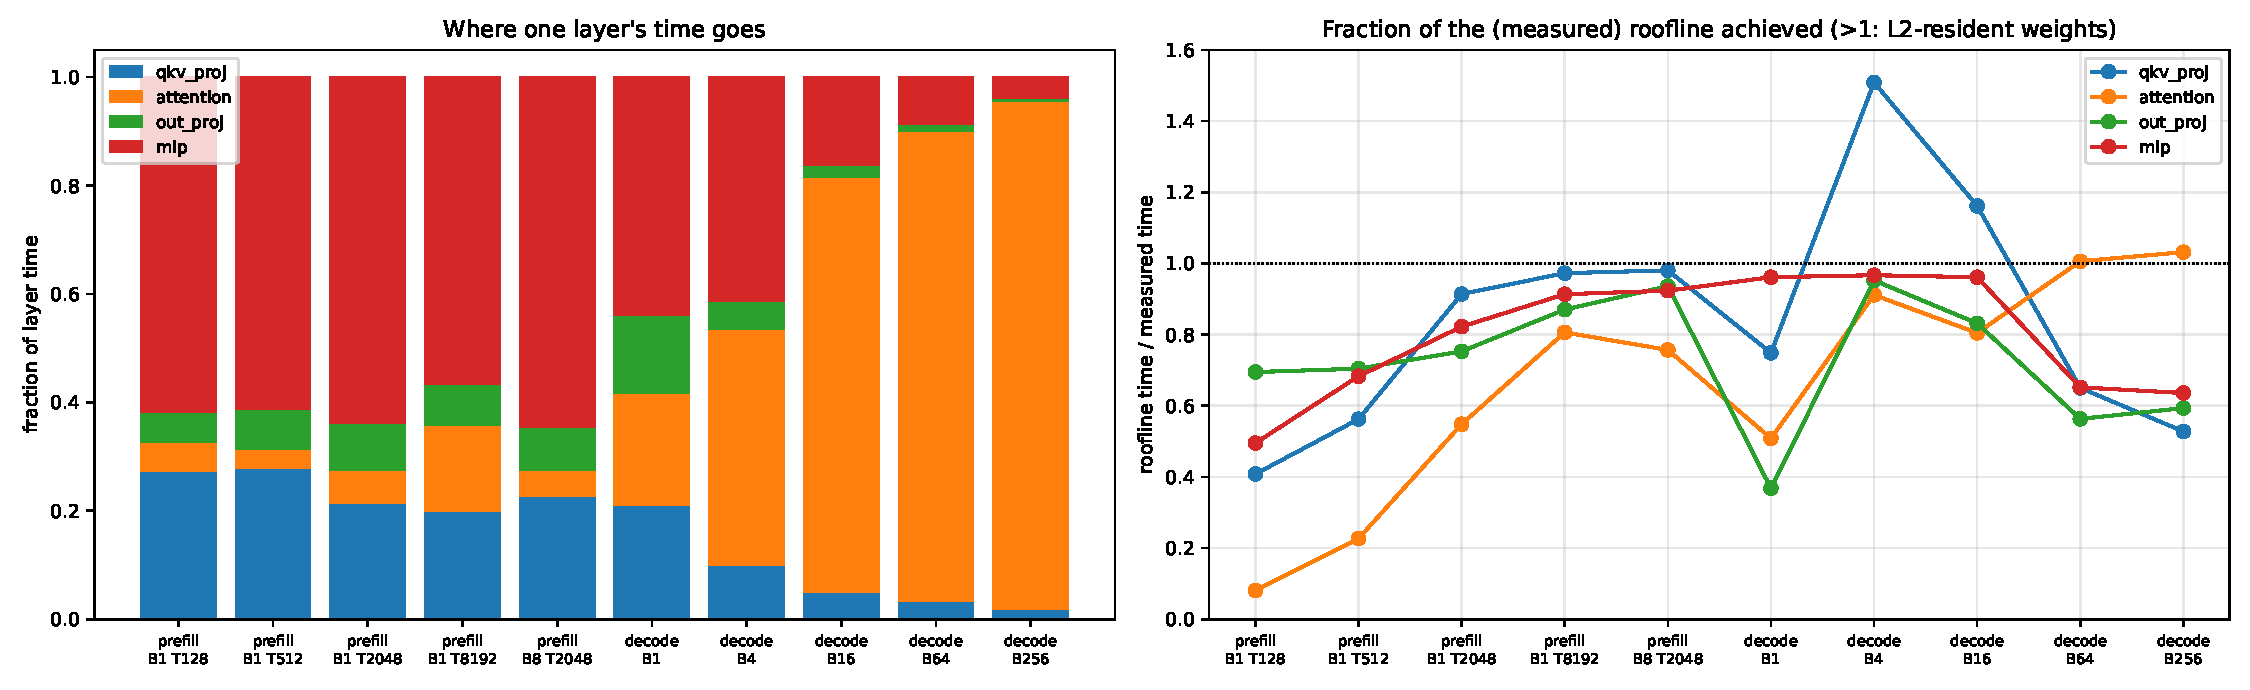
\includegraphics[width=\linewidth]{gpu_layer_breakdown.pdf}
\caption{左：一层时间在四个算子间的分配；右：各算子达到的 roofline 比例。}
\label{fig:breakdown}
\end{figure}

\Cref{fig:breakdown}：decode $B=1$ 时一层 0.420 ms，MLP 占 44\%（它的权重最多）；decode $B=256$ 时 attention 占 94\%（10.95 / 11.67 ms），因为投影的权重读取被 256 个序列摊薄，而 KV cache 读取没有。
这就是为什么长上下文、大 batch 的 decode 需要 GQA/MQA 或 KV 量化，而不是更快的矩阵乘。prefill $T=8192$ 时 attention 只占 16\%（2.887 / 18.08 ms），MLP 占 57\%。
按 decode $B=1$ 一层 0.420 ms 估算，32 层约 13.4 ms/token（不含 LM head），对应约 74 token/s；纯权重读取下界是 13.5 GB ÷ 1.522 TB/s = 8.9 ms。

\subsection{Depthwise 卷积}\label{sec:conv}

\begin{figure}[H]
\centering
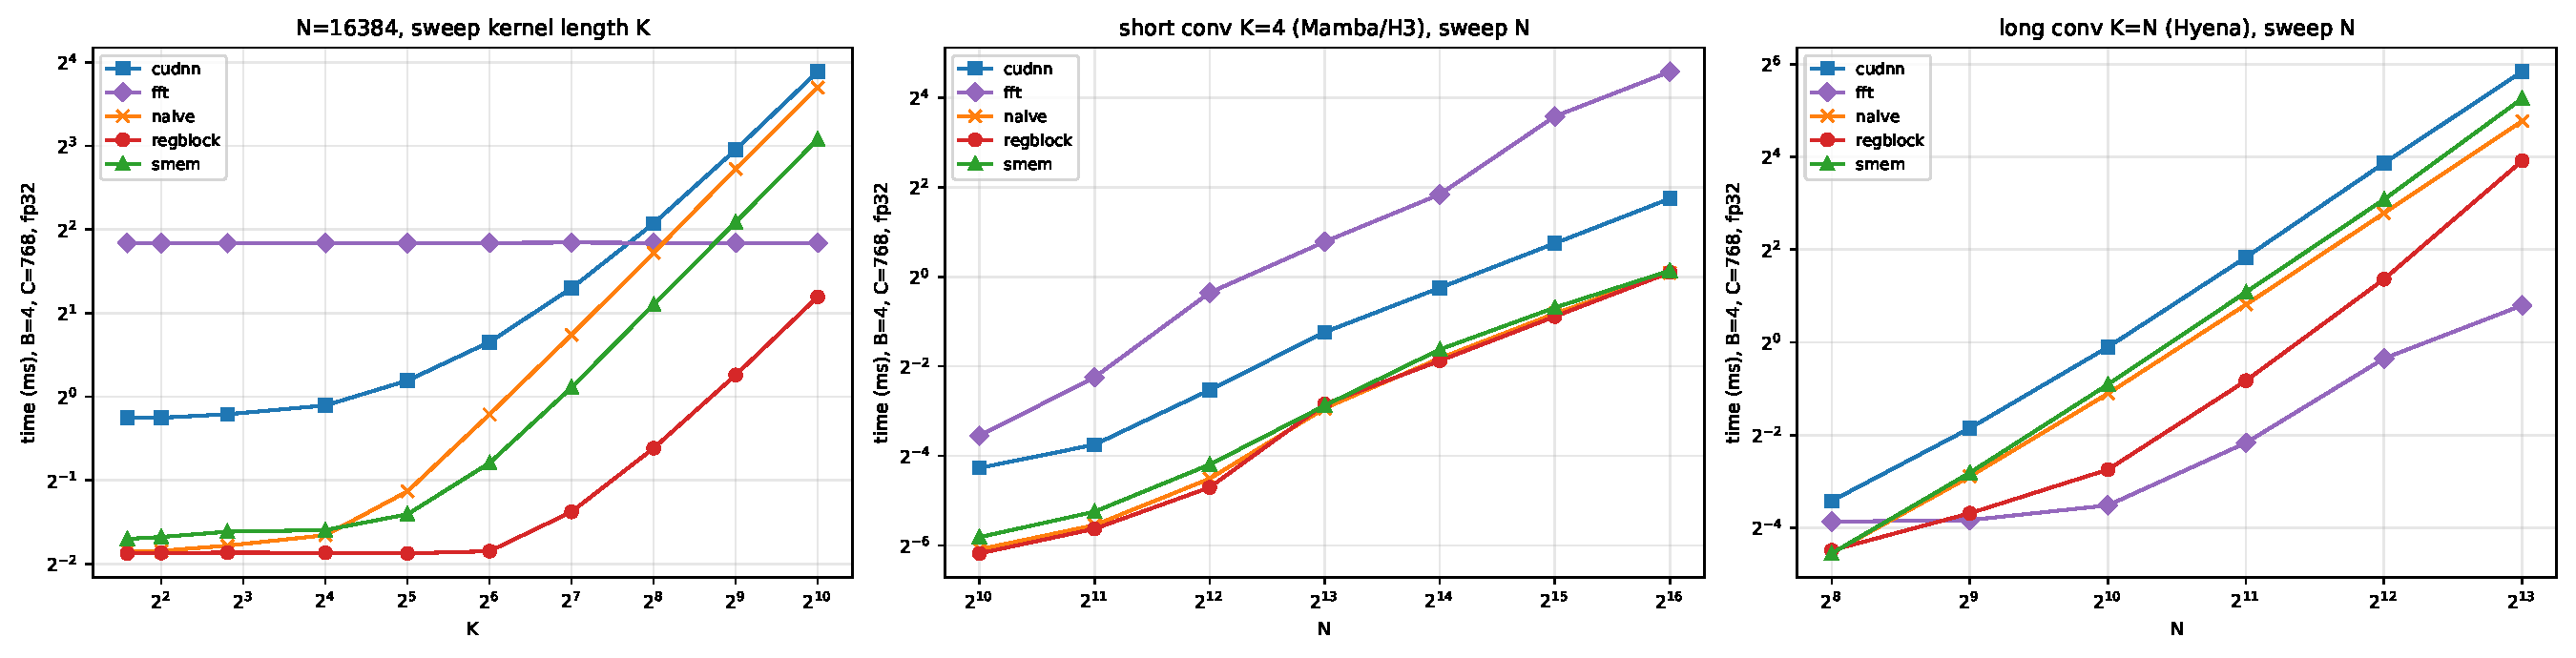
\includegraphics[width=\linewidth]{gpu_dwconv_time.pdf}
\caption{Depthwise 因果卷积（$B=4$，$C=768$，fp32；\texttt{dwconv.jsonl}）。左：$N=16384$ 扫 $K$；中：$K=4$ 扫 $N$；右：$K=N$ 扫 $N$。}
\label{fig:conv}
\end{figure}

\begin{table}[H]
\centering\small
\caption{Depthwise 卷积耗时（ms，$B=4,C=768$，fp32）}\label{tab:conv}
\begin{tabular}{lrrrrr}
\toprule
设置 & naive & smem & regblock & cuDNN & FFT \\
\midrule
$N=16384,K=4$ & 0.2785 & 0.3124 & \textbf{0.2735} & 0.8396 & 3.577 \\
$N=16384,K=64$ & 0.8633 & 0.5770 & \textbf{0.2776} & 1.573 & 3.581 \\
$N=16384,K=1024$ & 13.00 & 8.462 & \textbf{2.289} & 14.82 & 3.581 \\
$K=N=512$ & 0.1343 & 0.1423 & 0.0776 & 0.2768 & \textbf{0.0701} \\
$K=N=4096$ & 6.900 & 8.463 & 2.569 & 14.57 & \textbf{0.7851} \\
$K=N=8192$ & 27.28 & 38.20 & 15.07 & 57.18 & \textbf{1.737} \\
\bottomrule
\end{tabular}
\end{table}

正确性：三个 kernel 与 fp64 cuDNN 参考的最大误差随 $K$ 增长（累加项变多），$K=4$ 时 8.0e-7，$K=1024$ 时 7.9e-6，$K=4096$ 时 1.4e-5；FFT 约 2.5e-6。

\Cref{fig:conv,tab:conv}：
\textbf{短卷积（$K\le32$）是纯访存问题}。$K=4$ 时三个 kernel 都在 0.27–0.31 ms，regblock 1472 GB/s，达到 copy 带宽的 97\%；
cuDNN 慢 3.07 倍（480 GB/s），它对 depthwise 1D 没有专门路径。$N\le4096$ 时数据（$4\times768\times4096\times4=50$ MB）能放进 L2，带宽超过 DRAM（$N=4096$：2624 GB/s）。
\textbf{长卷积（$K\ge128$）变成计算问题}。$K=1024$ 时 regblock 2.289 ms，等效 45.0 TFLOP/s，是 naive 的 5.7 倍、smem 的 3.7 倍、cuDNN 的 6.5 倍。
\textbf{与 FFT 的交叉点}：$N=16384$ 时 FFT 恒为 3.58 ms，regblock 在 $K=1024$ 时仍快 1.56 倍，线性外推交叉点约 $K\approx1600$；
$K=N$ 时 FFT 从 $N=512$ 起更快（0.0701 对 0.0776 ms），$N=8192$ 时快 8.7 倍。CPU 上 $N=16384$ 时交叉点是 $K\approx16$–$64$，GPU 上右移了 25–100 倍：GPU 的 FMA 吞吐与带宽之比远高于 CPU，而 FFT 是访存受限的。

\begin{figure}[H]
\centering
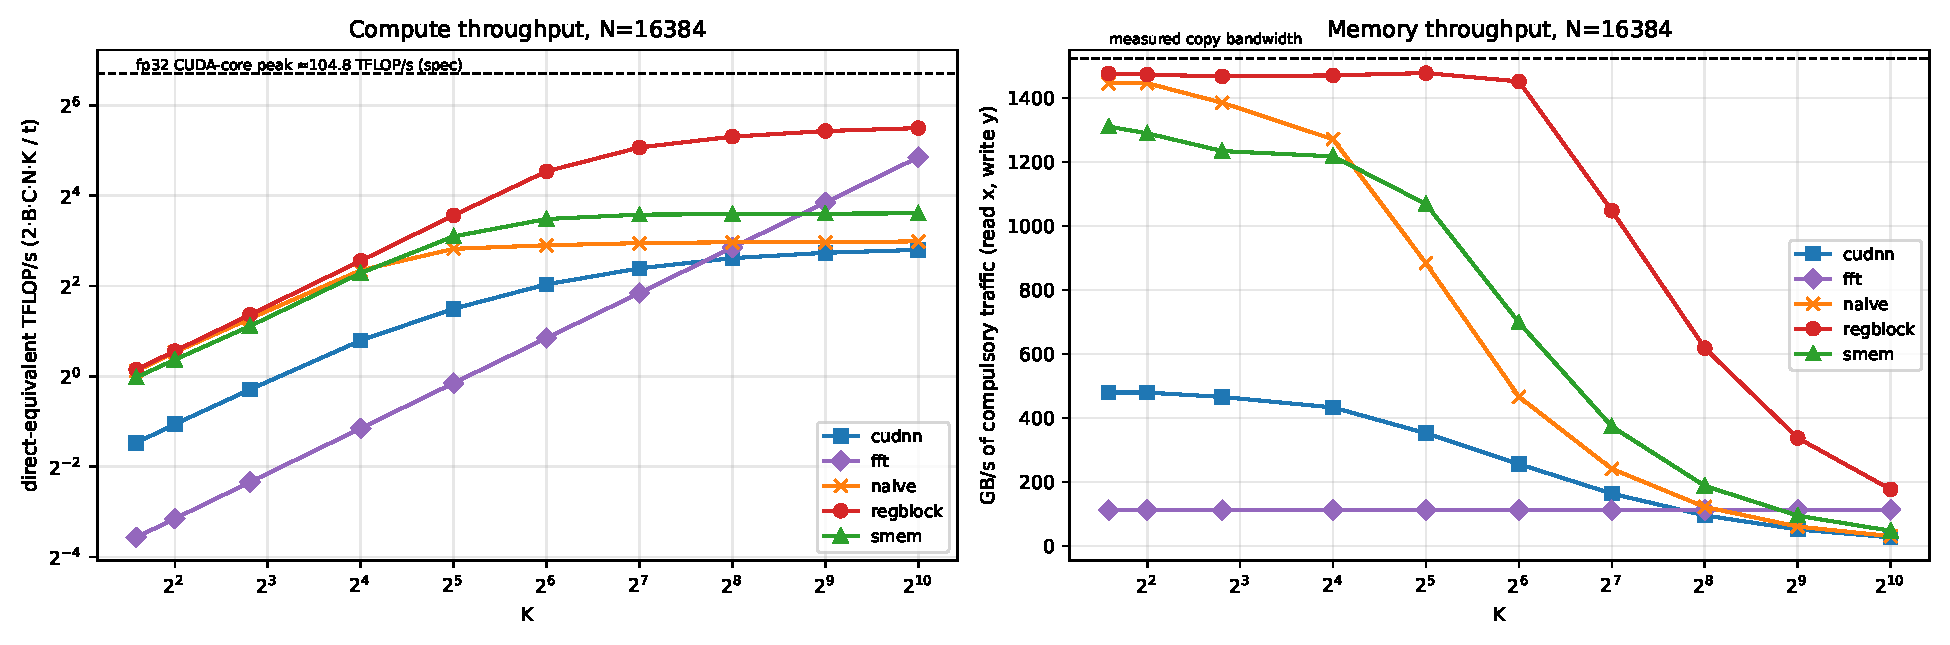
\includegraphics[width=\linewidth]{gpu_dwconv_throughput.pdf}
\caption{$N=16384$ 时的计算吞吐（直接卷积等效 FLOPs）与必需访存吞吐（读 $x$、写 $y$）。}
\label{fig:convtp}
\end{figure}

\Cref{fig:convtp} 左图中 smem kernel 在 $K\ge128$ 时停在 12.0–12.2 TFLOP/s，naive 停在 7.7–7.9 TFLOP/s。smem 的平台可以用共享内存带宽解释：
每个 FMA（2 FLOP）要 2 次 4 字节共享内存读，即 4 B/FLOP；共享内存带宽约 $170\text{ SM}\times32\text{ bank}\times4\text{ B}\times2.6\text{ GHz}\approx56.6$ TB/s，上限约 14 TFLOP/s，实测 12.2 是它的 86\%。
regblock 每 64 个 FMA 只要 23 次读（$h$ 8 次广播、$x$ 15 次），即 0.72 B/FLOP，共享内存上限升到约 79 TFLOP/s，实测 45.0 TFLOP/s 已接近 fp32 CUDA core 规格峰值（104.8）的一半。
这就是「寄存器分块」的全部意义：把共享内存读取次数从 $O(RK)$ 降到 $O(K\cdot 3R/R)$，让瓶颈回到 FMA 单元。

\subsection{训练：MQAR 与吞吐}\label{sec:train}

\paragraph{MQAR：先找一个学得会的设置。}
第一次尝试（$n_k=256$、$P=32$、lr $10^{-3}$、wd 0.1，4000 步）准确率停在约 5\%，于是做了两轮扫描（\cref{fig:mqarsweep}，\texttt{train\_mqar\_sweep*.jsonl}）。
eval 准确率（$16\times512$ 条新序列）：

\begin{table}[H]
\centering\small
\caption{MQAR 扫描（2 层，bf16 + SDPA）。}
\label{tab:mqarsweep}
\begin{tabular}{rrrrrr}
\toprule
$n_k$ & $P$ & lr & wd & 步数 & eval 准确率 \\
\midrule
64 & 4 & $10^{-3}$ & 0 & 6000 & \textbf{1.000} \\
64 & 8 & $10^{-3}$ & 0 & 6000 & \textbf{1.000} \\
64 & 8 & $3\times10^{-3}$ & 0.1 & 6000 & 0.364 \\
64 & 8 & $3\times10^{-3}$ & 0 & 2000 & 0.361 \\
64 & 16 & $10^{-3}$ & 0.1 & 6000 & 0.253 \\
64 & 16 & $3\times10^{-3}$ & 0 & 2000 & 0.250 \\
128 & 16 & $10^{-3}$ & 0.1 & 6000 & 0.231 \\
256 & 32 & $3\times10^{-3}$ & 0 & 2000 & 0.101 \\
256 & 32 & $10^{-3}$ & 0.1 & 4000 & 约 0.05 \\
\bottomrule
\end{tabular}
\end{table}

两点规律：(1) 学会是「全有或全无」——要么 1.000，要么卡在一个明显低于 1 的平台；(2) 学习率比步数更关键：$P=8$ 时 lr $3\times10^{-3}$ 跑 6000 步仍停在 0.36，lr $10^{-3}$ 在第 1000 步左右就跳到 1.0。
$P=16$ 在 6000 步内两种 lr 都没有跳出平台。

\begin{figure}[H]
\centering
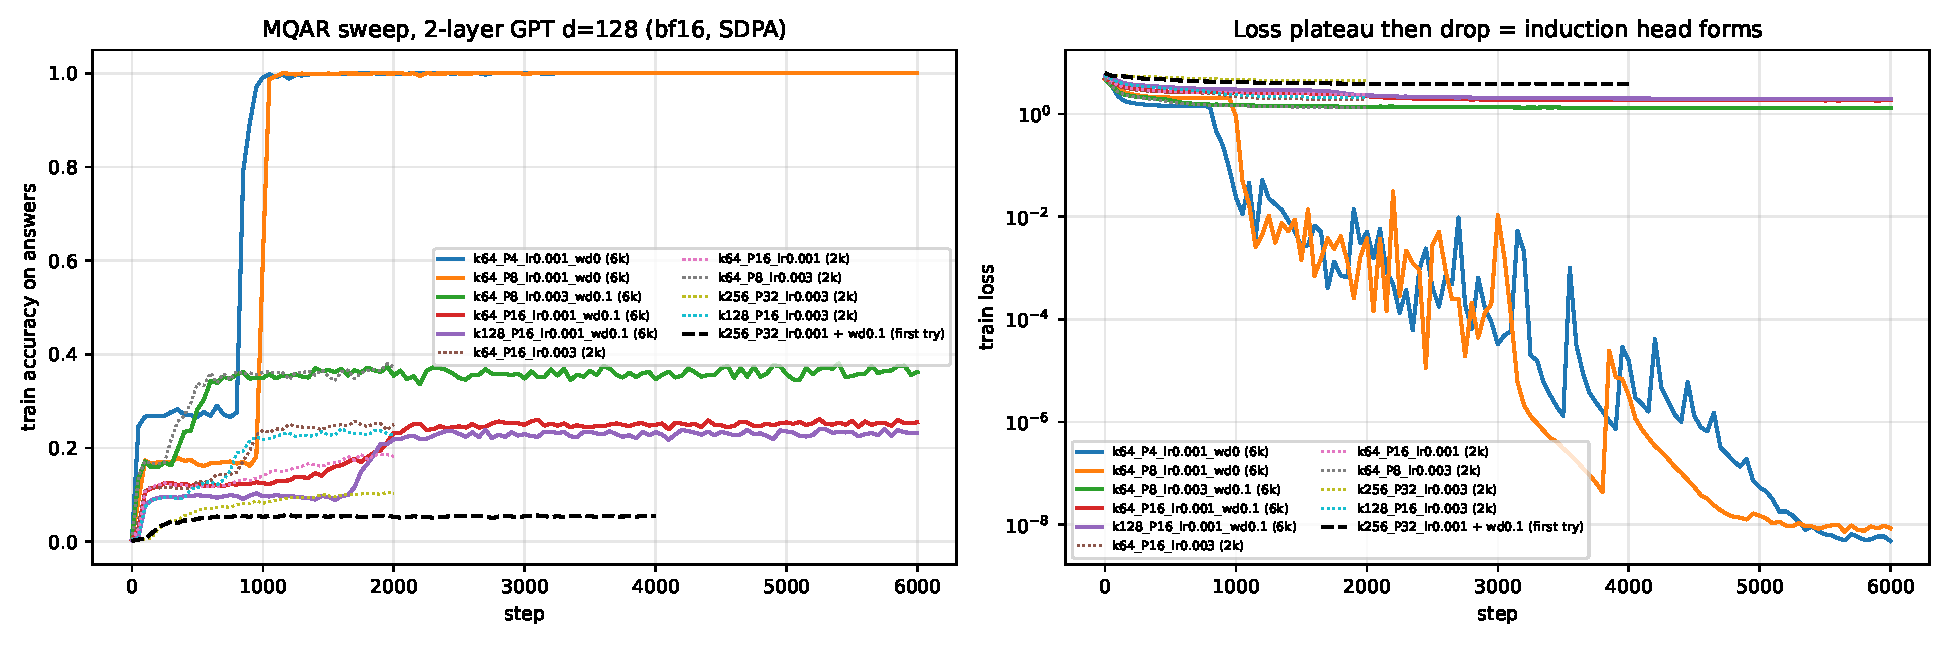
\includegraphics[width=\linewidth]{gpu_mqar_sweep.pdf}
\caption{MQAR 扫描的训练准确率与 loss。实线为 6000 步一轮，点线为 2000 步一轮，黑虚线为第一次尝试。学会的设置都是先停在平台，再在几十步内跳到 100\%。}
\label{fig:mqarsweep}
\end{figure}

\paragraph{MQAR 对照实验。}
选出的设置是 $n_k=64$、$P=8$（$T=32$）、lr $10^{-3}$、wd 0，每种配置 6000 步、同一个种子（\texttt{train\_mqar.jsonl}，\cref{fig:mqar}）：

\begin{table}[H]
\centering\small
\caption{MQAR 对照（$n_k=64$，$P=8$，6000 步，batch 256）。}
\label{tab:mqar}
\begin{tabular}{lrrrrr}
\toprule
配置 & 参数量 & eval 准确率 & 首次 acc$\ge$0.99 & 训练时间 (s) & tokens/s \\
\midrule
2 层，bf16 + SDPA & 413k & 1.000 & 第 1100 步 & 63.5 & 0.77 M \\
1 层，bf16 + SDPA & 215k & 0.172 & — & 44.8 & 1.10 M \\
2 层，bf16 + Triton（本文） & 413k & 1.000 & 第 1100 步 & 75.1 & 0.65 M \\
2 层，fp32 + 朴素 & 413k & 1.000 & 第 1100 步 & 63.2 & 0.78 M \\
\bottomrule
\end{tabular}
\end{table}

\begin{figure}[H]
\centering
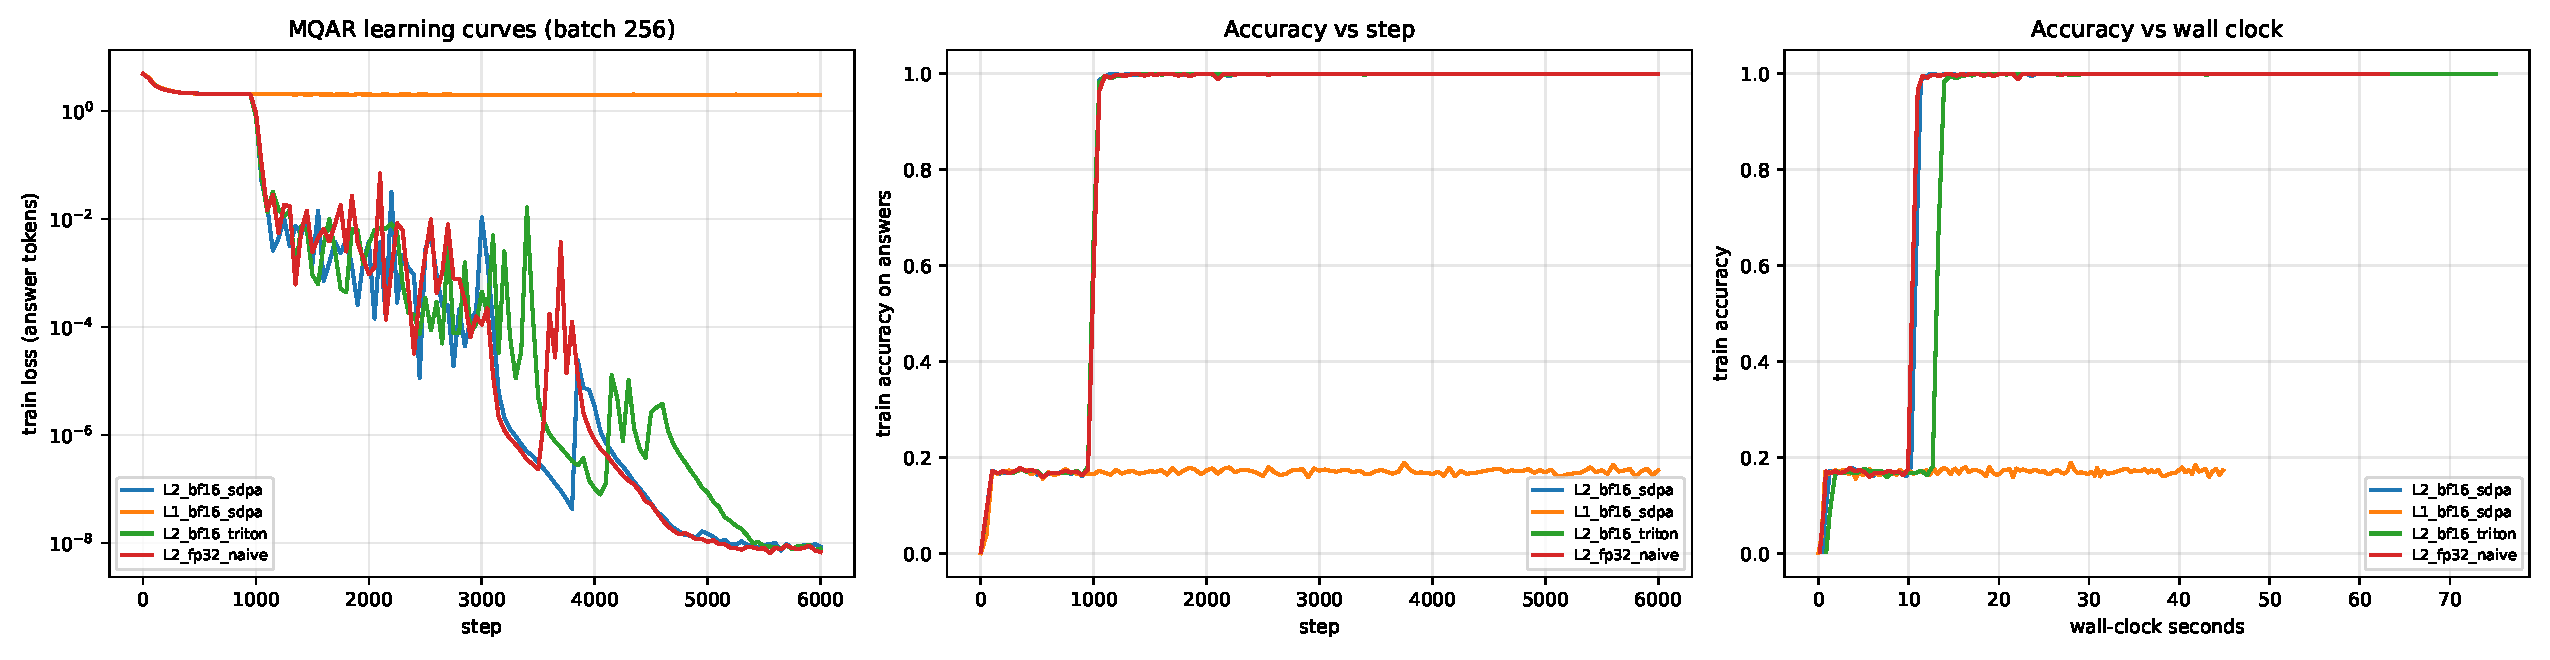
\includegraphics[width=\linewidth]{gpu_mqar_curves.pdf}
\caption{MQAR 学习曲线（按步数与按墙钟时间）。三个 2 层模型的曲线在第 1000 步前几乎重合，都先停在与 1 层模型相同的 0.17 平台，然后同时跳到 100\%。}
\label{fig:mqar}
\end{figure}

\begin{itemize}
\item \textbf{1 层学不会，2 层在第 1000–1100 步突然学会}。2 层模型在前 1000 步的准确率与 1 层模型一样停在约 0.17，然后在 100 步内跳到 1.0，loss 从 2.0 掉到 $10^{-2}$ 以下。
  0.17 略高于 $1/P=0.125$：只靠一层 attention，模型能学到「从上下文里出现过的 value 中挑一个」（高于 $1/P$ 的部分可能来自排除已回答过的 value，这里没有验证），但无法把查询与对应的 key 匹配。
  匹配需要两步：先让每个 value 位置通过上一 token 头记住它前面的 key，再让查询去匹配这个 key——这正是 \cref{sec:cpu} 手写构造与 induction head\cite{induction} 的结构，它至少需要两层。
\item \textbf{三种 attention 实现学到同一个结果}：bf16 + SDPA、bf16 + 本文 Triton kernel（前向 + 反向）、fp32 + 朴素实现都在第 1100 步首次达到 0.99，最终都是 1.000。
  这是 Triton 反向在真实训练中的端到端校验：如果 dQ/dK/dV 有错，学习曲线不会与 SDPA 重合。之后 loss 曲线的差别（Triton 在 $10^{-4}$–$10^{-6}$ 区间下降稍慢）来自 bf16 的舍入路径不同，不影响准确率。
\item \textbf{这个规模下实现选择不影响速度}：$T=32$、$d=128$ 的模型每步只有约 10 ms，几乎全是 kernel 启动开销；fp32 朴素与 bf16 SDPA 一样快（0.78 对 0.77 M tokens/s），Triton 慢 18\%，因为它的反向要多启动一个求 $\delta$ 的 torch kernel 和两个 Triton kernel，并经过 \texttt{autograd.Function} 的 Python 开销。
\end{itemize}

\paragraph{吞吐与 MFU。}
GPT-2-small 形状（110.2M 参数，不含位置编码；$T=1024$，$B=8$，每步 8192 tokens），每种配置 3 步预热后取 10 步（\texttt{train\_throughput.jsonl}，\cref{fig:train,tab:train}）。

\begin{table}[H]
\centering\small
\caption{GPT-2-small 形状训练吞吐（$T=1024$，$B=8$）。MFU 分母为实测 BF16 峰值 236.3 TFLOP/s。}
\label{tab:train}
\begin{tabular}{llrrrrr}
\toprule
精度 & attention & 每步 (ms) & k tokens/s & MFU（$6N$） & MFU（$+12LTd$） & 峰值显存 (GB) \\
\midrule
fp32 & 朴素 & 197.3 & 41.5 & 0.116 & 0.136 & 15.38 \\
fp32 & SDPA & 137.5 & 59.6 & 0.167 & 0.195 & 10.53 \\
TF32 & 朴素 & 158.0 & 51.9 & 0.145 & 0.170 & 15.38 \\
TF32 & SDPA & 99.6 & 82.2 & 0.230 & 0.270 & 10.54 \\
bf16 & 朴素 & 126.4 & 64.8 & 0.181 & 0.213 & 15.37 \\
bf16 & SDPA & \textbf{51.3} & \textbf{159.6} & \textbf{0.447} & \textbf{0.523} & 8.27 \\
bf16 & Triton（本文） & 52.5 & 156.0 & 0.437 & 0.512 & 8.25 \\
\bottomrule
\end{tabular}
\end{table}

\begin{figure}[H]
\centering
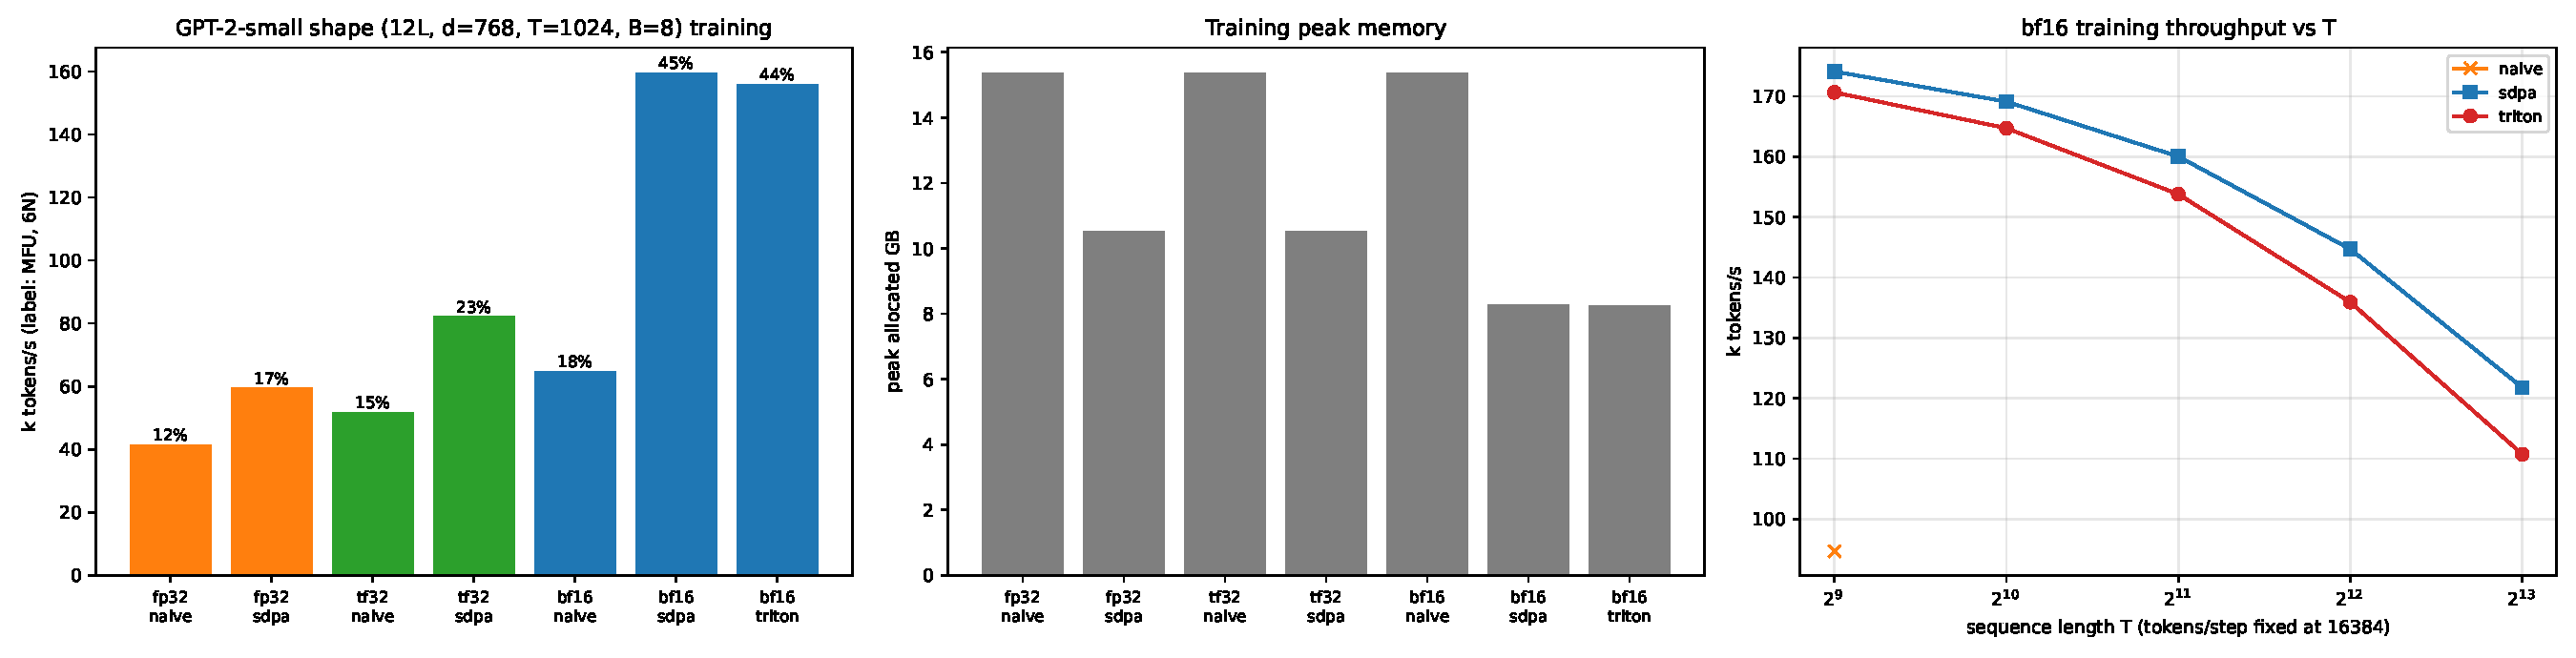
\includegraphics[width=\linewidth]{gpu_train_throughput.pdf}
\caption{左：吞吐与 MFU（柱上数字）；中：峰值显存；右：固定每步 16384 tokens 时吞吐随 $T$ 的变化（朴素实现从 $T=1024$、$B=16$ 起 OOM）。}
\label{fig:train}
\end{figure}

\begin{itemize}
\item \textbf{bf16 autocast 与 flash attention 需要一起用}：只开 bf16（朴素 attention）只快 1.56 倍（41.5k → 64.8k），只换 SDPA（fp32）只快 1.44 倍；两者一起快 3.84 倍（159.6k）。
  原因是朴素 attention 的 $T^2$ 分数张量（$B\cdot H\cdot T^2=8\times12\times1024^2$ 个元素，每层要存 softmax 输入输出供反向）是访存受限的，bf16 只能把这部分字节减半，而矩阵乘部分 bf16 才是 tensor core 的主场。
\item \textbf{显存}：SDPA 把峰值从 15.4 GB 降到 8.3 GB（bf16），省下的正是每层保存的 $T^2$ 张量；每步 16384 tokens（$T=1024$、$B=16$）时 bf16 朴素实现已经 OOM（显存 32 GB）。
\item \textbf{本文的 Triton kernel 达到 SDPA 的 97.7\%}（156.0k 对 159.6k）。前向基本持平，差距来自反向（\cref{fig:bwd}：反向是 PyTorch FA2 的 80\%）。
\item \textbf{MFU}：bf16 + SDPA 达到 0.447（$6N$），计入 attention 后 0.523。剩下的约一半时间花在 LayerNorm、GELU、残差、交叉熵（词表 32768）和 AdamW 等访存受限的操作上。
\item \textbf{序列长度}：固定每步 16384 tokens，SDPA 吞吐从 $T=512$ 的 174.1k 降到 $T=8192$ 的 121.8k，因为 attention FLOPs 随 $T$ 线性增长；按 $6N$ 的 MFU 随之降到 0.34，但按 PaLM 公式计入 attention 后升到 0.81。
  PaLM 的 $12LTd$ 计的是非因果的全部 attention FLOPs，因果 kernel 只算一半；按 $6LTd$ 修正后，MFU 在 $T=512$–8192 间稳定在 0.51–0.57。Triton 在 $T=8192$ 时为 110.7k（SDPA 的 91\%），长序列下反向差距更明显。
\end{itemize}

\subsection{手写 associative recall 在 GPU 上的复核}\label{sec:recallgpu}

把 CPU 部分的手工权重模型直接放到 GPU（\texttt{train\_recall.jsonl}）：4 种键值对数 $\times$ 6 个 $\beta$ 共 24 组、每组 5000 条序列（与 CPU 实验相同的随机种子），
GPU 与 CPU 的准确率逐格相同，预测不一致数为 0（例如 32 对、$\beta=4$：两者都是 0.9988；$\beta=1$：都是 0.2268）。
每组 5000 条在 GPU 上前向约 0.7–4 ms（第一次调用含 CUDA 初始化，193 ms）。这说明 \cref{fig:cpu-recall} 的构造与设备无关，fp32 下 $\beta=30$ 的 softmax 也没有数值问题。

%======================================================================
\section{与理论模型的对照}\label{sec:theory}
%======================================================================

\subsection{Attention 的 FLOPs、字节与强度}
单头前向 FLOPs：$QK^\top$ 与 $PV$ 各 $2T^2d$，共 $4T^2d$（因果有用部分减半）。字节（fp16，2 B/元素）：
\begin{align}
\text{朴素（教科书）}&: 2(4Td+4T^2) & I&=\frac{4T^2d}{8T^2}=\frac{d}{2},\\
\text{朴素（eager）}&: 2(4Td+6T^2) & I&=\frac{4T^2d}{12T^2}=\frac{d}{3},\\
\text{Flash}&: 2\left(2Td+\frac{T}{B_r}\cdot 2Td\right) & I&\approx\frac{4T^2d}{4T^2d/B_r}=B_r.\label{eq:flashI}
\end{align}
朴素实现 $d=64$ 的强度是 21.3 FLOP/B，远低于 ridge 155，按 roofline 预测吞吐 $1.522\text{ TB/s}\times21.3=32.5$ TFLOP/s，实测 30.1（$T=8192$），误差 7\%；
$d=128$ 时预测 65.0、实测 51.7。因果 eager 实现多了 \texttt{masked\_fill} 的一读一写（$8T^2$）而有用 FLOPs 减半，$I=d/8=8$，预测 12.2、实测 8.7 TFLOP/s。

\Cref{eq:flashI} 是一个面试中很好用的结论：\textbf{FlashAttention 前向的 DRAM 强度等于 Q 块的行数 $B_r$}（fp16）。$B_r=128$ 时 $I=128<155$，按模型它应当略低于计算屋顶（$1.522\times128=195$ TFLOP/s），
实测 215–224 TFLOP/s 超过了这个值——又一次说明 L2 让实际 DRAM 字节少于模型。论文中的 $\Theta(T^2d^2/M)$ 就是把 $B_r\propto M/d$ 代入 $T^2d/B_r$ 得到的；
在 sm\_120 上 $M\approx99$ KB，$B_r$ 被寄存器容量限制在 128 左右，因此在 $d=64$–$128$ 时它仍然是 $\Theta(T^2)$，只是常数比朴素实现小 $\frac{3B_r}{d}$ 倍（eager 计数）。

\subsection{为什么 FlashAttention 快：三个因素的分解}
以 $d=64$、$T=8192$、非因果为例（Triton 2.558 ms，朴素 18.28 ms，比值 7.15）：
\begin{enumerate}
\item 朴素实现是访存受限的，时间 $\approx 25.90\text{ GB}/1.522\text{ TB/s}=17.0$ ms，占实测 18.28 ms 的 93\%；
\item flash 是计算受限的，时间 $\approx 4\cdot32\cdot8192^2\cdot64/236.3\text{ TFLOP/s}=2.33$ ms，占实测 2.558 ms 的 91\%；
\item 所以加速比 $\approx \frac{\text{bytes}_{\text{eager}}/BW}{\text{FLOPs}/\text{peak}}=\frac{6T^2\cdot2/BW}{4T^2d/\text{peak}}=\frac{3\cdot\text{ridge}}{d}=\frac{3\times155.3}{64}=7.3$，与实测 7.15 吻合。
\end{enumerate}
这个式子同时解释了 $d=128$ 时加速比更小（$\frac{3\times155.3}{128}=3.6$，实测 21.26/5.617=3.8），以及因果时加速比更大（朴素多读写一次且算满 $T^2$，flash 跳过一半块）。

\subsection{Roofline 中的线性层}
\texttt{gemm\_intensity}$(M,N,K)=\frac{2MNK}{2(MK+KN+MN)}$。decode 时 $M=B\ll N,K$，$I\approx\frac{2BNK}{2NK}=B$；ridge 155 意味着 batch 要超过约 155 才能让投影变成计算受限，这与实测 $B=256$ 的 QKV 投影（$I=236$）首次越过 ridge 一致。
与 \texttt{mlsys\_calc.critical\_batch} 的思路相同：临界 batch $\approx$ ridge $\times$ 每元素字节 / 2。
decode attention 的强度 $\frac{4Hd_hT}{2\cdot2Hd_hT}=1$，与 batch、上下文长度无关；GQA-8\cite{gqa}（Llama-3-8B）把它提高到 4，MQA\cite{mqa} 到 32，但仍低于 ridge，所以 GQA 的收益是「读更少的字节」而非「变成计算受限」。

\subsection{卷积}
直接卷积 FLOPs $2BCNK$，必需字节 $4(2BCN+CK)$，强度 $\approx K/4$。$K=4$、$N=16384$ 时 $I=1$，访存受限：必需字节 $4(2\cdot4\cdot768\cdot16384+768\cdot4)=402.7$ MB，
按 copy 带宽预测 0.265 ms，实测 regblock 0.2735 ms（1472 GB/s，97\%）。
$K=1024$ 时 $I=256$，按 DRAM 是计算受限，但真正的瓶颈是片上（共享内存）带宽，见 \cref{sec:conv} 的推导。
FFT 卷积的 FLOPs 只有 $O(N\log N)$，但要对长度 $2N$ 的复数数组做多遍读写，是访存受限的；GPU 的 FLOP/字节之比（ridge）比 CPU 高得多，
直接卷积多出来的 FLOPs 很便宜，所以交叉点 $K^{*}$ 大幅右移。

%======================================================================
\section{面试专题}
%======================================================================

\paragraph{20 秒电梯陈述}
我在 RTX 5090 上用 Triton 写了 FlashAttention-2 的前向和反向。前向在 $T=16$k 时跑到 224 TFLOP/s，是实测矩阵乘峰值的 95\%，和 PyTorch 自带的 FA2 持平，比朴素实现快 7 倍（因果 22 倍），显存从 8.6 GB 降到 35 MB。
我用 roofline 把加速比拆成了一个公式：朴素实现以 93\% 的 DRAM 带宽运行，flash 以 91\% 的算力运行，所以加速比约等于 $3\times\text{ridge}/d$。我还发现教科书的 IO 模型在 GPU 上高估 DRAM 流量最多 4 倍，因为 K/V 重读命中了 96 MB 的 L2。

\paragraph{STAR 故事}
\textbf{S}：课程作业只要求 numpy 版的 FlashAttention，CPU 上它比朴素实现还慢（$T=1024$ 时 44.6 对 22.9 ms），IO 模型也只说它少 2 倍流量，很难说明为什么工业界都用它。
\textbf{T}：在真实 GPU 上量化「到底快多少、为什么快」，并检验 IO 模型。
\textbf{A}：写 Triton 前向/反向并用 fp32 参考验证（35 个 GPU 测试）；扫 $T$、$d$、因果、dtype 和 $B_r\times B_c$；实测 copy 带宽和矩阵乘峰值，把每个实现的时间换算成「隐含带宽」和「算力利用率」。
\textbf{R}：前向 224.0 TFLOP/s，与 SDPA flash（217.9）持平；朴素 OOM 点在 $T=16384$（两个 fp16 $T\times T$ 张量 34 GB）；用 $3\cdot\text{ridge}/d=7.3$ 预测出实测 7.15 倍的加速；
块扫描中隐含带宽 6.57 TB/s 证明了 L2 复用。反向只有 FA2 的 80\%，我能定位到原因是两 kernel 结构多做了 2 个矩阵乘。

\begin{iqbox}{FlashAttention 到底省了什么？流量是不是降了一个阶？}
省的首先是显存：不物化 $T\times T$ 的 $S$、$P$，额外显存从 $O(T^2)$ 降到 $O(T)$（$T=8192$：8.62 GB → 34.6 MB）。流量是 $\Theta(T^2d^2/M)$，在 $d=64$–$128$、$B_r$ 被 SRAM/寄存器封顶时仍是 $\Theta(T^2)$，只是常数小 $3B_r/d$ 倍；
真正的时间收益来自「把访存受限的程序变成计算受限的程序」：加速比 $\approx3\cdot\text{ridge}/d$。
\tcblower
\textbf{常见错答}：「FlashAttention 把 attention 从 $O(T^2)$ 变成 $O(T)$。」——计算量仍是 $4T^2d$，没有任何近似。
\end{iqbox}

\begin{iqbox}{FlashAttention 前向的算术强度是多少？}
fp16 下约等于 Q 块的行数 $B_r$：每个 Q 块读整段 K/V（$4Td$ 字节）并做 $4B_rTd$ FLOPs。$B_r=128$ 时 $I\approx128$，接近 5090 的 ridge 155。所以 $B_r$ 不能太小（$B_r=16$ 时吞吐只有一半），也不能太大（寄存器溢出，$B_r=256$ 下降）。
\tcblower
\textbf{常见错答}：「强度和 $T$ 成正比，所以序列越长越计算受限。」——每个 Q 块对每个 K/V 元素只用一次，强度与 $T$ 无关。
\end{iqbox}

\begin{iqbox}{为什么朴素 attention 在 GPU 上只有 30 TFLOP/s？}
它的强度是 $d/3\approx21$ FLOP/B（eager 实现：matmul 写 $S$、scale 读写、softmax 读写、matmul 读 $P$，共 $6T^2$ 次 fp16 访问），远低于 ridge 155；按 1.522 TB/s 预测 32.5 TFLOP/s，实测 30.1。
\tcblower
\textbf{常见错答}：「因为 softmax 很慢。」——softmax 只是其中两次 $T^2$ 访问，换成任何逐元素操作都一样慢；问题是物化 $T\times T$ 的中间结果。
\end{iqbox}

\begin{iqbox}{online softmax 为什么正确？反向为什么只存 lse？}
维护 $m'=\max(m,s)$，$\ell'=\ell e^{m-m'}+\sum e^{s-m'}$，$\mathrm{acc}'=\mathrm{acc}\,e^{m-m'}+e^{s-m'}V$；任意时刻 $\mathrm{acc}/\ell$ 都等于已见 key 上的精确 softmax 加权和。
反向用 $P=\exp(S-\mathrm{lse})$ 重算，一个标量 $\mathrm{lse}=m+\log\ell$ 就够，比存 $m,\ell$ 两个量省显存，也省一次除法。本文用以 2 为底的版本，\texttt{exp2} 是单条 SFU 指令。
\tcblower
\textbf{常见错答}：「online softmax 是近似的。」——它是精确的重排，误差只来自浮点舍入（fp16 下 6.6e-5，与 PyTorch FA2 相同）。
\end{iqbox}

\begin{iqbox}{decode 阶段加大 batch 能让 attention 变成计算受限吗？}
不能。decode attention 的强度 $=2(H/H_{kv})/b$，MHA 时为 1，与 batch 和上下文都无关：每个序列有自己的 KV cache。实测 $B=1\to256$ 强度一直是 1.00，$B=256$ 时 attention 占一层时间的 94\%。
batch 只对线性层有用（强度 $\approx B$），$B\approx155$ 才越过 ridge。
\tcblower
\textbf{常见错答}：「batch 越大 GPU 利用率越高，所以 decode 都应该开大 batch。」——对 attention 无效；要靠 GQA/MQA、KV 量化或 PagedAttention 提高可容纳的 batch。
\end{iqbox}

\begin{iqbox}{IO 模型说 flash 流量是朴素的 1/2（或 1/6），为什么 GPU 上测不到这个比例？}
三个原因：(1) eager 朴素实现的 $T^2$ 访问是 6 次不是 4 次；(2) GPU kernel 的 $B_r=128$ 大于 CPU 模型里的 $B_r=d=64$；(3) K/V 重读大量命中 L2——块扫描中按模型算的隐含带宽高达 6.57 TB/s，是 DRAM 的 4.3 倍。
而且 flash 是计算受限的，时间比本就不等于字节比。
\tcblower
\textbf{常见错答}：「模型错了。」——模型给的是 DRAM 流量的上界，它在 SRAM 只有一级、没有 L2 的假设下是对的。
\end{iqbox}

\begin{iqbox}{depthwise 卷积什么时候用 FFT？}
直接卷积 $O(NK)$、强度约 $K/4$；FFT $O(N\log N)$ 但访存受限。GPU 上 $N=16384$ 时交叉点约 $K\approx1600$（$K=1024$ 时寄存器分块 kernel 2.29 ms 仍快于 FFT 3.58 ms），$K=N$ 时 $N\ge512$ 用 FFT。CPU 上交叉点是 $K\approx16$–$64$。
所以 Mamba/H3 的短卷积（$K=4$）直接写，Hyena 的长卷积（$K=N$）用 FFT。
\tcblower
\textbf{常见错答}：「$K>\log N$ 就用 FFT。」——这是只数 FLOPs 的结论；GPU 上直接卷积的 FLOPs 很便宜，FFT 的访存更贵。
\end{iqbox}

\begin{iqbox}{共享内存 tiling 为什么在长卷积上只快 1.5 倍？寄存器分块解决了什么？}
smem 版每个 FMA 仍要 2 次共享内存读（4 B/FLOP），共享内存带宽约 57 TB/s，上限约 14 TFLOP/s，实测 12.2。寄存器分块每 64 FMA 读 23 次（0.72 B/FLOP），上限升到约 79，实测 45.0 TFLOP/s，比 smem 快 3.7 倍。
还要处理 stride-8 访问的 8 路 bank 冲突（填充下标 \texttt{i+(i>>5)}）和输出的合并写。
\tcblower
\textbf{常见错答}：「共享内存和寄存器一样快，搬进共享内存就够了。」——共享内存带宽比寄存器低一个数量级，高复用的 kernel 必须在寄存器层再分块。
\end{iqbox}

\begin{iqbox}{为什么 cuDNN 的 depthwise conv1d 比手写 naive 还慢？}
$K=4$ 时 cuDNN 0.840 ms，naive 0.279 ms。cuDNN 的卷积主要为 2D、通道混合的卷积优化（implicit GEMM），depthwise 1D（groups=C）没有专门路径，还要先 \texttt{F.pad} 复制一次输入（额外一读一写）。
这也是 Mamba/H3 都自己写 \texttt{causal\_conv1d} kernel 的原因。
\tcblower
\textbf{常见错答}：「库一定比手写快。」——库只对它优化过的形状快。
\end{iqbox}

\begin{iqbox}{MFU 怎么算？为什么小模型 MFU 低？}
$\text{MFU}=6N\cdot\text{tokens/s}/\text{peak}$（\texttt{mlsys\_calc.mfu}），$6N$ 是每 token 前向 $2N$、反向 $4N$ 的 FLOPs，不含 attention 的 $12LTd$。分母用实测 BF16 峰值 236.3 TFLOP/s。
小模型（$d=128$）的矩阵乘太小，启动开销和逐元素操作（LayerNorm、GELU、优化器）占主导；GPT-2-small 形状的数字见 \cref{sec:train}。
\tcblower
\textbf{常见错答}：「MFU 低说明 GPU 坏了 / kernel 写得差。」——MFU 低首先是形状问题；也不能用 fp32 的 MFU 与 bf16 峰值直接比较而不说明。
\end{iqbox}

%======================================================================
\section{局限}
%======================================================================

\begin{caveatbox}
\begin{itemize}
\item \textbf{没有直接测量 DRAM 字节}：容器无权读取性能计数器（ncu 报 \texttt{ERR\_NVGPUCTRPERM}），所有「流量」结论都是模型字节 ÷ 实测时间得到的隐含带宽。L2 复用是由隐含带宽超过 DRAM 峰值推断出来的，没有给出命中率。
\item \textbf{不能推出「Triton kernel 比 PyTorch FA2 更快」}：只在 $T\ge8192$、$d=64$ 时快 2–4\%，短序列和 $d=128$ 时更慢，反向只有 80\%；且 PyTorch 的 FA2 未必针对 sm\_120 调过优。
\item \textbf{不能推出 decode 小 batch 投影能超过 roofline}：$B=4$ 的 eff 1.51 来自重复测量时权重留在 L2，真实推理逐层轮换权重。
\item \textbf{只测了单卡、单层}：没有测通信、整模型的 kernel 融合、CUDA graph；层内 MLP 的 \texttt{silu}$\cdot$ 是单独的逐元素 kernel，没有融合。
\item \textbf{共享 GPU}：计时在共享锁内独占完成，但 CPU 只有 2 个核，主机侧开销（如 Triton 反向在短序列上约 0.53 ms 的平台）比独占机器大。
\item \textbf{卷积 kernel 只做了 fp32 前向}，没有 bf16、没有反向，也没有像 \texttt{causal\_conv1d} 那样对 $K\le4$ 做专门的向量化路径。
\item \textbf{MQAR 结果只有一个随机种子}，学习曲线的转折步数可能随种子变化；任务规模很小（$P\le8$ 学得会，$P=16$ 在 6000 步内学不会），不能外推到 Zoology 论文中的长序列设置。
\item \textbf{「计入 attention 的 MFU」按 PaLM 的 $12LTd$ 计}，即非因果的全部 attention FLOPs；因果 kernel 跳过一半，按 $6LTd$ 计时 $T=8192$ 的 0.81 应为 0.57。
\end{itemize}
\end{caveatbox}

%======================================================================
\section{结论}
%======================================================================

\begin{findingbox}[：FlashAttention]
Triton FA2 前向 224.0 TFLOP/s（$T=16384$，$d=64$），为实测峰值的 95\%，与 PyTorch FA2 持平；比朴素实现快 7.15 倍（因果 22.2 倍），额外显存从 8.62 GB 降到 34.6 MB；朴素与 math 后端在 $T=16384$ 时 OOM。
加速比可由 $3\cdot\text{ridge}/d$ 预测（7.3 对实测 7.15）。
\end{findingbox}

\begin{findingbox}[：IO 模型]
教科书 IO 模型是 DRAM 流量的上界：朴素 eager 实现的 $6T^2$ 模型解释了 93\% 的耗时，而 flash 的模型字节对应的隐含带宽最高 6.57 TB/s（DRAM 的 4.3 倍），说明 K/V 重读主要由 96 MB L2 承担。flash 前向的 DRAM 强度约等于 $B_r$。
\end{findingbox}

\begin{findingbox}[：Roofline]
5090 实测 1.522 TB/s、236.3 TFLOP/s，ridge 155 FLOP/B。decode attention 强度恒为 1，$B=256$ 时占一层 94\% 的时间并以 1.57 TB/s 运行；decode 线性层强度 $\approx B$；prefill 全部算子计算受限，QKV 投影达到 97\% 的屋顶。
\end{findingbox}

\begin{findingbox}[：卷积]
寄存器分块 kernel 在 $K=4$ 时达到 copy 带宽的 97\%，在 $K=1024$ 时达到 45.0 TFLOP/s，比 cuDNN 快 6.5 倍、比 smem 版快 3.7 倍；GPU 上 FFT 的交叉点（$N=16384$ 时 $K\approx1600$）比 CPU 右移 25–100 倍。
\end{findingbox}

\begin{findingbox}[：训练]
MQAR（$n_k=64$，$P=8$）上 2 层 GPT 在第 1000–1100 步从 0.17 的平台突然跳到 100\%，1 层模型 6000 步仍停在 0.172；SDPA、本文 Triton kernel、fp32 朴素实现的学习曲线在跳变前完全重合，这是 Triton 反向的端到端校验。学习率比步数更关键（lr $3\times10^{-3}$ 卡在 0.36）。
GPT-2-small 形状训练中 bf16 + SDPA 达到 159.6k tokens/s、MFU 0.447（计入 attention 0.523），是 fp32 朴素实现的 3.84 倍，峰值显存从 15.4 GB 降到 8.3 GB；本文 Triton kernel 达到其 97.7\%。
\end{findingbox}

\begin{thebibliography}{99}
\bibitem{fa1} T. Dao, D. Y. Fu, S. Ermon, A. Rudra, C. Ré. FlashAttention: Fast and Memory-Efficient Exact Attention with IO-Awareness. NeurIPS 2022.
\bibitem{fa2} T. Dao. FlashAttention-2: Faster Attention with Better Parallelism and Work Partitioning. ICLR 2024.
\bibitem{online} M. Milakov, N. Gimelshein. Online normalizer calculation for softmax. arXiv:1805.02867, 2018.
\bibitem{rabe} M. N. Rabe, C. Staats. Self-attention Does Not Need $O(n^2)$ Memory. arXiv:2112.05682, 2021.
\bibitem{roofline} S. Williams, A. Waterman, D. Patterson. Roofline: An Insightful Visual Performance Model for Multicore Architectures. CACM 52(4), 2009.
\bibitem{triton} P. Tillet, H. T. Kung, D. Cox. Triton: An Intermediate Language and Compiler for Tiled Neural Network Computations. MAPL 2019.
\bibitem{h3} D. Y. Fu, T. Dao, K. K. Saab, A. W. Thomas, A. Rudra, C. Ré. Hungry Hungry Hippos: Towards Language Modeling with State Space Models. ICLR 2023.
\bibitem{hyena} M. Poli et al. Hyena Hierarchy: Towards Larger Convolutional Language Models. ICML 2023.
\bibitem{mamba} A. Gu, T. Dao. Mamba: Linear-Time Sequence Modeling with Selective State Spaces. arXiv:2312.00752, 2023.
\bibitem{zoology} S. Arora, S. Eyuboglu, A. Timalsina, I. Johnson, M. Poli, J. Zou, A. Rudra, C. Ré. Zoology: Measuring and Improving Recall in Efficient Language Models. ICLR 2024.
\bibitem{induction} C. Olsson et al. In-context Learning and Induction Heads. Transformer Circuits Thread, 2022.
\bibitem{palm} A. Chowdhery et al. PaLM: Scaling Language Modeling with Pathways. JMLR 24, 2023（附录 B：MFU 定义）.
\bibitem{gqa} J. Ainslie et al. GQA: Training Generalized Multi-Query Transformer Models from Multi-Head Checkpoints. EMNLP 2023.
\bibitem{mqa} N. Shazeer. Fast Transformer Decoding: One Write-Head is All You Need. arXiv:1911.02150, 2019.
\bibitem{flashdecoding} T. Dao, D. Haziza, F. Massa, G. Sizov. Flash-Decoding for long-context inference. PyTorch blog, 2023.
\bibitem{llama2} H. Touvron et al. Llama 2: Open Foundation and Fine-Tuned Chat Models. arXiv:2307.09288, 2023.
\end{thebibliography}

\end{document}
